%% ============================================================
%%  NanoAOD photon trigger objects: the unseeded diphoton leg
%%  Beamer / pdflatex, dark-beamer style
%%  Content from NOTES.md, results/REPORT.md and the HTML decks of the
%%  nanoaod-trigobj-notes branch (santanumahata/cmssw), 4-5 November 2026.
%% ============================================================
\documentclass[aspectratio=169,10pt]{beamer}

\usepackage[T1]{fontenc}
\usepackage[utf8]{inputenc}
\usepackage{lmodern}
\usepackage{graphicx}
\usepackage{booktabs}
\usepackage{array}
\usepackage{xcolor}
\usepackage{amsmath}
\usepackage{amssymb}
\usepackage{microtype}
\usepackage{hyperref}
\usepackage{tikz}
\usetikzlibrary{arrows.meta, positioning, fit, backgrounds, calc}
\usetikzlibrary{decorations.pathmorphing, decorations.markings}
\usepackage{pgfplots}\pgfplotsset{compat=1.16}
\usepackage{listings}
\usepackage{tabularx}
\usepackage{colortbl}
\usepackage{seqsplit}

\graphicspath{{../plots/}}   % <-- point at your figure directory

% ── Colour palette (CMS dark-navy style) ─────────────────────
\definecolor{navydark}  {RGB}{10,  27, 56}
\definecolor{navymid}   {RGB}{18,  48, 96}
\definecolor{cmsblue}   {RGB}{ 0, 112,192}
\definecolor{cmsaccent} {RGB}{ 0, 188,235}
\definecolor{cmsgold}   {RGB}{255,185,  0}
\definecolor{lightgrey} {RGB}{210,220,235}
\definecolor{offwhite}  {RGB}{240,244,250}

\newcommand{\shorttitletext}{NanoAOD photon TrigObj: unseeded diphoton leg \quad$\cdot$\quad S. Mahata, 5 November 2026}

% ── Beamer theme setup ───────────────────────────────────────
\usetheme{default}
\setbeamertemplate{navigation symbols}{}
\setbeamertemplate{itemize item}{\color{cmsaccent}\small$\blacktriangleright$}
\setbeamertemplate{itemize subitem}{\color{cmsgold}\footnotesize$\bullet$}
\setbeamercolor{background canvas}{bg=navydark}
\setbeamercolor{normal text}{fg=offwhite}
\setbeamercolor{alerted text}{fg=cmsgold}
\setbeamercolor{example text}{fg=cmsaccent}
\setbeamercolor{frametitle}{fg=cmsaccent, bg=navymid}
\setbeamerfont{frametitle}{size=\large, series=\bfseries}
\setbeamertemplate{frametitle}{%
  \vskip2pt
  \hspace*{6pt}\insertframetitle
  \vskip3pt
  \color{cmsaccent}\rule{\linewidth}{0.4pt}%
  \vskip2pt
}
\setbeamercolor{structure}{fg=cmsaccent}
\setbeamercolor{item}{fg=cmsaccent}
\setbeamercolor{subitem}{fg=cmsgold}
\setbeamercolor{footline}{fg=lightgrey, bg=navymid}
\setbeamertemplate{footline}{%
  \begin{beamercolorbox}[wd=\paperwidth,ht=2.2ex,dp=1ex]{footline}
    \hspace*{6pt}\tiny \shorttitletext
    \hfill \tiny\insertframenumber\,/\,\inserttotalframenumber\hspace*{6pt}
  \end{beamercolorbox}%
}
\setbeamercolor{block title}{fg=navydark, bg=cmsaccent}
\setbeamercolor{block body}{fg=navydark, bg=offwhite}
\setbeamercolor{block title alerted}{fg=navydark, bg=cmsgold}
\setbeamercolor{block body alerted}{fg=navydark, bg=offwhite}
\hypersetup{colorlinks=true, urlcolor=cmsaccent, linkcolor=cmsaccent}

% ── Macros ───────────────────────────────────────────────────
\newcommand{\pT}{\ensuremath{p_{\mathrm{T}}}}
\newcommand{\etal}{\ensuremath{|\eta|}}
\newcommand{\Hgg}{\ensuremath{H\!\to\!\gamma\gamma}}
\newcommand{\Zee}{\ensuremath{Z\!\to\!ee}}
\newcommand{\RNine}{\ensuremath{R_{9}}}
\newcommand{\hl}[1]{\textcolor{cmsaccent}{\textbf{#1}}}
\newcommand{\gold}[1]{\textcolor{cmsgold}{\textbf{#1}}}
\newcommand{\plotslide}[3][0.80]{%
  \begin{center}
    \includegraphics[width=#1\linewidth,height=0.74\textheight,keepaspectratio]{#2}\\[2pt]
    {\tiny\color{lightgrey}#3}
  \end{center}}

% ── White frame (for CMS public plots on white canvas) ───────
\newenvironment{whiteframe}[1]{%
  \setbeamercolor{background canvas}{bg=white}%
  \setbeamercolor{normal text}{fg=navydark}%
  \setbeamercolor{frametitle}{fg=navymid, bg=white}%
  \setbeamertemplate{frametitle}{\vskip2pt\hspace*{6pt}\insertframetitle\vskip3pt
    \color{navymid}\rule{\linewidth}{0.4pt}\vskip2pt}%
  \setbeamercolor{footline}{fg=navymid, bg=white}%
  \usebeamercolor[fg]{normal text}%
  \begin{frame}{#1}}{\end{frame}}
\newcommand{\whitecap}[1]{{\tiny\color{navymid}#1}}
\newcommand{\TODO}[1]{\textcolor{cmsgold}{$\langle$\,TODO: #1\,$\rangle$}}
\newcommand{\partdivider}[2]{%
  {\setbeamercolor{background canvas}{bg=navymid}
   \setbeamertemplate{footline}{}
   \begin{frame}[plain]
     \vspace*{2.0cm}\centering
     \ifx&#1&\else{\large\color{lightgrey} #1}\\[8pt]\fi
     {\huge\bfseries\color{cmsaccent} #2}
   \end{frame}}}


% ── Additions for this deck ──────────────────────────────────
\newcommand{\code}[1]{\texttt{\detokenize{#1}}}            % identifiers with underscores
\newcommand{\fname}[1]{{\ttfamily\seqsplit{#1}}}           % long filter names, breakable anywhere
\newcommand{\dead}[1]{\textcolor{cmsgold}{\textbf{#1}}}
\newcommand{\src}[1]{\vfill{\tiny\color{lightgrey}#1}}
\lstdefinestyle{dark}{basicstyle=\ttfamily\fontsize{6.2}{7.2}\selectfont\color{offwhite},
  backgroundcolor=\color{navymid}, frame=single, rulecolor=\color{cmsaccent}, framesep=3pt,
  keywordstyle=\color{cmsaccent}, commentstyle=\color{lightgrey}\itshape, stringstyle=\color{cmsgold},
  columns=fullflexible, keepspaces=true, showstringspaces=false, breaklines=true,
  breakatwhitespace=false, xleftmargin=3pt, xrightmargin=3pt, aboveskip=2pt, belowskip=2pt,
  upquote=true, literate={γ}{{$\gamma$}}1 {→}{{$\to$}}1}
\lstset{style=dark}
\lstdefinestyle{codebk}{style=dark, basicstyle=\ttfamily\fontsize{5.0}{5.85}\selectfont\color{offwhite},
  numbers=left, numberstyle=\tiny\color{lightgrey}, numbersep=4pt, xleftmargin=12pt, firstnumber=auto,
  morekeywords={}, aboveskip=1pt, belowskip=0pt}
\newcolumntype{Y}{>{\raggedright\arraybackslash}X}
\arrayrulecolor{cmsaccent}
\renewcommand{\arraystretch}{1.12}
\newcommand{\thead}[1]{\textcolor{cmsaccent}{\textbf{#1}}}
\newcommand{\rowdead}{\rowcolor{navymid}}


\title{\textbf{The unseeded diphoton leg never gets its NanoAOD filter bits}}
\author{Santanu Mahata}
\date{5 November 2026}

\begin{document}

% ── Title page ───────────────────────────────────────────────
{
\setbeamertemplate{footline}{}
\begin{frame}[plain]
  \vspace*{0.9cm}
  \begin{center}
    {\footnotesize\color{cmsaccent} CMS $\cdot$ NanoAOD $\cdot$ trigger objects}\\[8pt]
    {\color{cmsaccent}\rule{0.7\linewidth}{1.5pt}}\\[10pt]
    {\Large\bfseries\color{white} The unseeded diphoton leg never gets}\\[6pt]
    {\Large\bfseries\color{white} its NanoAOD filter bits}\\[10pt]
    {\color{cmsaccent}\rule{0.7\linewidth}{1.5pt}}\\[12pt]
    {\small\color{lightgrey} Photon \code{TrigObj_filterBits} 16, 17 (14, 15 before NanoAOD v15) of
     \code{HLT_Diphoton30_22_R9Id_OR_IsoCaloId_AND_HE_R9Id_Mass90} / \code{Mass95}:\\
     documented, never set. Cause, scope, the one-line fix and its test on real input.}\\[16pt]
    {\large\color{white} Santanu Mahata}\\[4pt]
    {\footnotesize\color{cmsgold} 5 November 2026}\\[10pt]
    {\tiny\color{lightgrey} Checked against cms-sw/cmssw master ed35654b1, release branches 13\_0\_X to 16\_1\_X,
     HLT menus 2018 to 2026, thirteen NanoAOD files and NANO re-runs with the fix}
  \end{center}
\end{frame}
}

% ── Outline ──────────────────────────────────────────────────
\begin{frame}{Outline}
  \begin{enumerate}
    \item \hl{The problem} --- what a NanoAOD trigger object is, the diphoton path, where the object is dropped.
    \item \hl{Scope} --- every NanoAOD version since v12, every menu since 2018, thirteen files measured,
          a scan of the whole trigger-object table.
    \item \hl{Fix and validation} --- the one-line fix, the fix test on real MiniAOD input, trigger efficiency
          of the Diphoton30\_22 and Diphoton30\_18 unseeded legs, the relval in CMSSW\_16\_1\_3, impact on analyses,
          pull-request status.
    \item \hl{Backup} --- the code at every step, all tables, history, production recipe, reproducibility.
  \end{enumerate}
  \src{Repository: \url{https://github.com/santanumahata/cmssw/tree/nanoaod-trigobj-notes} (NOTES.md, results/REPORT.md, scripts/).}
\end{frame}

% =============================================================
\partdivider{Part I}{The problem}
% =============================================================

\begin{frame}{The problem in one page}
  \begin{columns}[T]
    \begin{column}{0.24\linewidth}\centering
      {\Huge\bfseries\color{cmsgold}3}\par\vspace{2pt}
      {\scriptsize photon filter bits documented but impossible to set (16, 17, 19 in v15; 14, 15, 17 in v12 to v14)}
    \end{column}
    \begin{column}{0.24\linewidth}\centering
      {\Huge\bfseries\color{cmsgold}4+}\par\vspace{2pt}
      {\scriptsize NanoAOD versions affected: v12, v13, v14, v15, 2026 data (16\_0\_X) and master}
    \end{column}
    \begin{column}{0.24\linewidth}\centering
      {\Huge\bfseries\color{cmsaccent}19}\par\vspace{2pt}
      {\scriptsize HLT menu files checked, 2018 to 2026: same filter names, same collections}
    \end{column}
    \begin{column}{0.24\linewidth}\centering
      {\Huge\bfseries\color{cmsaccent}1}\par\vspace{2pt}
      {\scriptsize line to change in \code{triggerObjects_cff.py}, as the Electron selection did in 2023}
    \end{column}
  \end{columns}
  \par\vspace{8pt}
  \begin{itemize}\small
    \item \gold{Problem}: the Photon entry of the trigger-object table accepts only objects from
          \code{hltEgammaCandidates}; the sub-leading leg of the Diphoton30\_22 Mass90/Mass95 paths is built on
          \code{hltEgammaCandidatesUnseeded}. The collection test runs before the bits are computed, so those
          objects are dropped and their bits can never appear.
    \item \gold{Measured}: thirteen NanoAOD files, v9 to v15 and 2026 data (16\_0\_X): not one photon object with an unseeded bit.
    \item \hl{Fix}: accept both collections in the Photon selection. NANO re-made with the fix sets the unseeded
          bits in all 10453 Mass90 events of the MC test file and in all 308 of a 2026 data test file (16\_0\_4\_patch2).
  \end{itemize}
  \src{NOTES.md sections 1, 7, 14, 15; results/REPORT.md.}
\end{frame}

\begin{frame}[fragile]{What a NanoAOD trigger object is, and how analyses use the filter bits}
  \begin{columns}[T]
    \begin{column}{0.56\linewidth}
      {\scriptsize
      \begin{tabularx}{\linewidth}{@{}lY@{}}
        \toprule
        \thead{branch} & \thead{meaning}\\\midrule
        \code{TrigObj_id} & object type: 11 electron, 22 photon, 13 muon, 15 tau, 1 jet, 6 fat jet, 2 MET, 3 HT, 4 MHT\\
        \code{TrigObj_pt, eta, phi} & HLT object kinematics (e/gamma: the supercluster)\\
        \code{TrigObj_l1pt, l1iso} & matched L1 seed in a cone (type $-98$ for e/gamma)\\
        \code{TrigObj_filterBits} & one bit per HLT filter passed, per-type list in \code{triggerObjects_cff.py};
          32-bit up to 15\_0\_1, 64-bit from 15\_0\_2\\\bottomrule
      \end{tabularx}}
    \end{column}
    \begin{column}{0.42\linewidth}
\begin{lstlisting}[language=Python]
# sketch of a NanoAOD trigger match (awkward)
to   = events.TrigObj
ph   = to[to.id == 22]
leg2 = ph[(ph.filterBits >> 17) & 1 == 1]
# unseeded R9 leg: always empty today
dr   = photons.metric_table(leg2)
ok   = ak.any(dr < 0.1, axis=2)
\end{lstlisting}
    \end{column}
  \end{columns}
  \par\vspace{6pt}
  {\small A leg-by-leg efficiency, a trigger-matched tag-and-probe, or a matching of both photons needs the bit of
  the last filter of each leg. The filter labels are not stored in NanoAOD: the bits are the only record.
  For the sub-leading leg of the diphoton triggers the bit is never set, so the match always fails.}
  \src{The table is filled by TriggerObjectTableProducer from the unpacked MiniAOD trigger objects; an object is
  written only if it passes its type's selection string and sets at least one bit of that type.}
\end{frame}

\begin{frame}[fragile]{Two e/gamma candidate collections at HLT: L1-seeded and unseeded}
  \begin{columns}[T]
    \begin{column}{0.49\linewidth}
      {\small\hl{\code{hltEgammaCandidates}} (seeded): superclusters only around L1 e/gamma candidates.
       Leading leg ($E_\mathrm{T}>30$\,GeV, L1 match) and almost every single-photon/electron path.}
\begin{lstlisting}
fragment.hltEgammaCandidates = cms.EDProducer(
  "EgammaHLTRecoEcalCandidateProducers",
  scHybridBarrelProducer = cms.InputTag(
    'hltParticleFlowSuperClusterECALL1Seeded',
    'hltParticleFlowSuperClusterECALBarrel' ), ...
\end{lstlisting}
    \end{column}
    \begin{column}{0.49\linewidth}
      {\small\gold{\code{hltEgammaCandidatesUnseeded}}: superclusters over the whole ECAL, no L1 requirement.
       Sub-leading object of double-object paths ($E_\mathrm{T}>22$\,GeV here).}
\begin{lstlisting}
fragment.hltEgammaCandidatesUnseeded = cms.EDProducer(
  "EgammaHLTRecoEcalCandidateProducers",
  scHybridBarrelProducer = cms.InputTag(
    'hltParticleFlowSuperClusterECALUnseeded',
    'hltParticleFlowSuperClusterECALBarrel' ), ...
\end{lstlisting}
    \end{column}
  \end{columns}
  \par\vspace{6pt}
  {\small Two producers, two collections, two distinct trigger objects even when they describe the same photon.
  The trigger summary, PAT and MiniAOD keep the collection name with each object; NanoAOD decides per object type
  which names it accepts, and that is where the photon table goes wrong.}
  \src{Both producers from CMSSW\_13\_3\_1\_patch1 HLT\_FULL\_cff.py; the only difference is the supercluster input.}
\end{frame}

\begin{frame}{One path, two legs, four last filters}
  \centering
  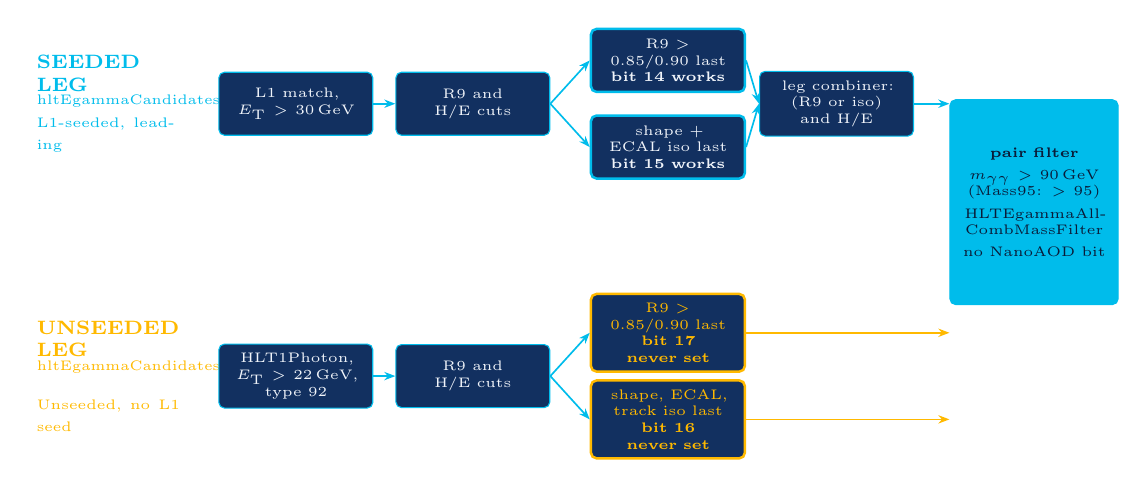
\begin{tikzpicture}[
      box/.style={draw=cmsaccent, fill=navymid, rounded corners=2pt, text=offwhite, font=\tiny,
                  align=center, minimum height=0.8cm, text width=1.72cm},
      goodbox/.style={box, draw=cmsaccent, line width=0.9pt},
      badbox/.style={box, draw=cmsgold, line width=0.9pt, text=cmsgold},
      endbox/.style={draw=cmsaccent, fill=cmsaccent, rounded corners=2pt, text=navydark, font=\tiny,
                  align=center, minimum height=2.6cm, text width=1.9cm},
      lab/.style={font=\scriptsize\bfseries, align=left, text width=1.9cm},
      arr/.style={-{Stealth[length=4pt]}, cmsaccent, line width=0.6pt},
      node distance=0.28cm]
    \node[lab, text=cmsaccent] (sl) {SEEDED LEG\\[-1pt]{\tiny\mdseries hltEgammaCandidates\\L1-seeded, leading}};
    \node[box, right=of sl] (s1) {L1 match,\\$E_\mathrm{T}>30$\,GeV};
    \node[box, right=of s1] (s2) {R9 and H/E cuts};
    \node[goodbox, right=0.5cm of s2, yshift=0.55cm] (s3) {R9 $>$ 0.85/0.90 last\\\textbf{bit 14 works}};
    \node[goodbox, right=0.5cm of s2, yshift=-0.55cm] (s4) {shape + ECAL iso last\\\textbf{bit 15 works}};
    \node[box, right=0.4cm of s2, xshift=2.25cm] (s5) {leg combiner:\\(R9 or iso) and H/E};
    \node[lab, text=cmsgold, below=1.9cm of sl] (ul) {UNSEEDED LEG\\[-1pt]{\tiny\mdseries hltEgammaCandidates-\\Unseeded, no L1 seed}};
    \node[box, right=of ul] (u1) {HLT1Photon,\\$E_\mathrm{T}>22$\,GeV, type 92};
    \node[box, right=of u1] (u2) {R9 and H/E cuts};
    \node[badbox, right=0.5cm of u2, yshift=0.55cm] (u3) {R9 $>$ 0.85/0.90 last\\\textbf{bit 17 never set}};
    \node[badbox, right=0.5cm of u2, yshift=-0.55cm] (u4) {shape, ECAL, track iso last\\\textbf{bit 16 never set}};
    \node[endbox, right=0.45cm of s5, yshift=-1.25cm] (p) {\textbf{pair filter}\\[2pt] $m_{\gamma\gamma}>90$\,GeV\\(Mass95: $>95$)\\[2pt] HLTEgammaAll-\\CombMassFilter\\[2pt] no NanoAOD bit};
    \draw[arr] (s1) -- (s2); \draw[arr] (s2.east) -- (s3.west); \draw[arr] (s2.east) -- (s4.west);
    \draw[arr] (s3.east) -- (s5.west); \draw[arr] (s4.east) -- (s5.west); \draw[arr] (s5.east) -- (p.west |- s5.east);
    \draw[arr] (u1) -- (u2); \draw[arr] (u2.east) -- (u3.west); \draw[arr] (u2.east) -- (u4.west);
    \draw[arr, cmsgold] (u3.east) -- (p.west |- u3.east); \draw[arr, cmsgold] (u4.east) -- (p.west |- u4.east);
  \end{tikzpicture}
  \par\vspace{6pt}
  {\scriptsize Gold: the unseeded last filters NanoAOD discards. Bits in v15 numbering; in v12 to v14 the same
  four last filters are bits 12, 13 (seeded) and 15, 14 (unseeded). Mass95 shares the whole sequence.}
  \src{Each last filter is wrapped in cms.ignore(): it runs and saves its objects but cannot stop the path.
  The chain is identical (same MD5 of the ordered filter list) in all nineteen menu files checked.}
\end{frame}

\begin{frame}{From the HLT filter to \texttt{TrigObj\_filterBits}: four hand-offs survive, the fifth drops the object}
  \centering
  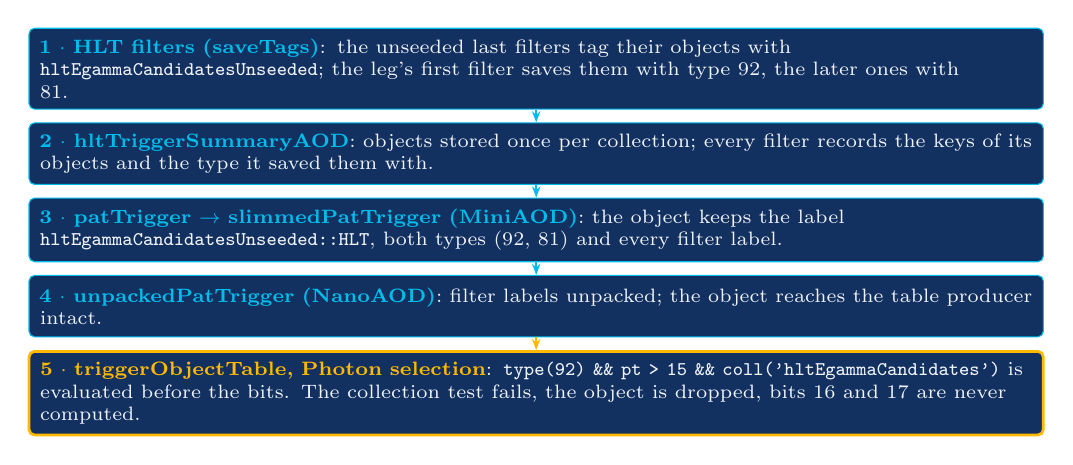
\begin{tikzpicture}[
      hstep/.style={draw=cmsaccent, fill=navymid, rounded corners=2pt, text=offwhite, font=\scriptsize,
                   align=left, text width=12.6cm, minimum height=0.78cm, inner sep=4pt},
      badstep/.style={hstep, draw=cmsgold, line width=1pt},
      arr/.style={-{Stealth[length=4pt]}, cmsaccent, line width=0.6pt}, node distance=0.16cm]
    \node[hstep] (a) {\hl{1 $\cdot$ HLT filters (saveTags)}: the unseeded last filters tag their objects with
      \code{hltEgammaCandidatesUnseeded}; the leg's first filter saves them with type 92, the later ones with 81.};
    \node[hstep, below=of a] (b) {\hl{2 $\cdot$ hltTriggerSummaryAOD}: objects stored once per collection; every
      filter records the keys of its objects and the type it saved them with.};
    \node[hstep, below=of b] (c) {\hl{3 $\cdot$ patTrigger $\to$ slimmedPatTrigger (MiniAOD)}: the object keeps the label
      \code{hltEgammaCandidatesUnseeded::HLT}, both types (92, 81) and every filter label.};
    \node[hstep, below=of c] (d) {\hl{4 $\cdot$ unpackedPatTrigger (NanoAOD)}: filter labels unpacked; the object reaches the
      table producer intact.};
    \node[badstep, below=of d] (e) {\gold{5 $\cdot$ triggerObjectTable, Photon selection}:
      \code{type(92) && pt > 15 && coll('hltEgammaCandidates')} is evaluated before the bits. The collection test
      fails, the object is dropped, bits 16 and 17 are never computed.};
    \draw[arr] (a) -- (b); \draw[arr] (b) -- (c); \draw[arr] (c) -- (d); \draw[arr, cmsgold] (d) -- (e);
  \end{tikzpicture}
  \src{The Electron selection has accepted hltEgammaCandidatesUnseeded since June 2023 and its unseeded CaloIdL\_MW
  bit is populated in production files: the objects are present up to the table producer.}
\end{frame}

\begin{frame}[fragile]{One unseeded photon object through the Photon selection, test by test}
  \begin{columns}[T]
    \begin{column}{0.52\linewidth}
      \begin{enumerate}\small
        \item \code{type(92)}: \hl{true}. \code{hltDiEG22EtEta2p55UnseededFilter} saved it with triggerType 92;
              PAT kept 92 next to the 81 of the later filters.
        \item \code{pt > 15}: \hl{true}. The leg requires 22\,GeV (18\,GeV for Diphoton30\_18).
        \item \code{coll('hltEgammaCandidates')}: \gold{false}. The label is
              \code{hltEgammaCandidatesUnseeded}; no wildcard, so an exact comparison.
        \item \code{sel.match(obj)} is false: the bits are never evaluated, the object is never written, bits 16
              and 17 are 0 in every event of every file.
      \end{enumerate}
    \end{column}
    \begin{column}{0.46\linewidth}
      {\scriptsize The Electron selection in the same file:}
\begin{lstlisting}
# CMSSW_13_0_13 (v12)
sel = "type(92) && pt > 7
  && coll('hltEgammaCandidates')
  && filter('*PixelMatchFilter')"
# CMSSW_13_3_0 onward (v13), PR 41827
sel = "type(92) && pt > 7
  && (coll('hltEgammaCandidates')
      || coll('hltEgammaCandidatesUnseeded'))
  && (filter('*PixelMatchFilter')
      || filter('*PixelMatchUnseededFilter'))"
\end{lstlisting}
    \end{column}
  \end{columns}
  \par\vspace{4pt}
  {\small PR 41827 (merged 8 June 2023) added the unseeded collection to the Electron selection. The diphoton photon
  bits had been added four months earlier by PR 40711 without that change.}
  \src{Backup frames give the code of every step: HLT1Photon, HLTGenericFilter, PATTriggerProducer, the slimmer,
  TriggerObjectTableProducer and TriggerObjectStandAlone::hasCollection.}
\end{frame}

% =============================================================
\partdivider{Part II}{Scope}
% =============================================================

\begin{frame}{Scope by NanoAOD version: present since the bits were added, still in master}
  \vspace{0pt}\par
  {\tiny
  \begin{tabularx}{\linewidth}{@{}lYp{2.3cm}p{1.9cm}p{1.6cm}l@{}}
    \toprule
    \thead{NanoAOD} & \thead{releases checked (tags and branch tips)} & \thead{Photon sel} & \thead{Electron sel} & \thead{dead photon bits} & \thead{affected}\\\midrule
    v9 & CMSSW\_10\_6\_X & seeded, pt$>$20, no bits & seeded & no photon TrigObj & no\\
    v10, v11 & CMSSW\_12\_4\_X, CMSSW\_12\_6\_X & seeded, pt$>$20, 12 bits & seeded & bits absent & no\\
    \rowdead v12 & 13\_0\_0 (pt$>$20), 13\_0\_1 to 13\_0\_17 (production 13\_0\_13) & seeded, 18 bits & seeded & 14, 15, 17 & \dead{yes}\\
    \rowdead v13 & 13\_3\_0, 13\_3\_1\_patch1 (production), 13\_3\_X tip & seeded, 18 bits & seeded + unseeded & 14, 15, 17 & \dead{yes}\\
    \rowdead v14 & 14\_0\_0, 14\_0\_X, 14\_1\_0, 14\_1\_X, 14\_2\_0, 14\_2\_X & seeded, 18 bits & seeded + unseeded & 14, 15, 17 & \dead{yes}\\
    \rowdead v15 & 15\_0\_2 to 15\_0\_15\_patch4, 15\_0\_X, 15\_1\_0, 15\_1\_X (15\_0\_0, 15\_0\_1: 18 bits) & seeded, 21 bits & seeded + unseeded & 16, 17, 19 & \dead{yes}\\
    \rowdead next & 16\_0\_10, 16\_0\_X, 16\_1\_3, 16\_1\_X, master ed35654b1 (4 Nov 2026) & seeded, 21 bits & seeded + unseeded & 16, 17, 19 & \dead{yes}\\\bottomrule
  \end{tabularx}}
  \par\vspace{2pt}
  \begin{itemize}\tiny
    \item Checked live on 4 November 2026: the Photon selection line is identical on master and on the tips of
          14\_1\_X to 16\_1\_X and at the newest tags CMSSW\_16\_1\_3 and CMSSW\_16\_0\_10.
    \item No open pull request or issue mentions hltEgammaCandidatesUnseeded, triggerObjects\_cff or photon trigger objects.
    \item Decimal values of the dead bits: 16384, 32768, 131072 (v12 to v14); 65536, 131072, 524288 (v15 and later).
  \end{itemize}
  \src{NOTES.md sections 7.2 and 13.1.}
\end{frame}

\begin{frame}{Scope by HLT menu: nine years of menus, the same four filters on the same collections}
  \vspace{0pt}\par
  {\scriptsize
  \begin{tabularx}{\linewidth}{@{}Yllp{3.6cm}@{}}
    \toprule
    \thead{menu (table name)} & \thead{Mass90/95} & \thead{Diphoton30\_18} & \thead{dead unseeded photon bits (v12--v14 / v15)}\\\midrule
    2018 GRun, /dev/CMSSW\_10\_6\_0/GRun/V3 & v13 & NoPixelVeto v2 & 14, 15, 17 / 16, 17, 19\\
    2022 frozen v1.2 (HLT\_2022v12, Run3Summer22 MC) & v13 & v2 & 14, 15, 17 / 16, 17, 19\\
    2022 frozen v1.4 and v1.5, GRun 12\_4 V171, GRun 12\_6 V16 & v15 & v3 & 14, 15, 17 / 16, 17, 19\\
    2023 frozen v1.2 (HLT\_2023v12), GRun 13\_0 V153 & v17 & v5 (renamed filters) & 14, 15 / 16, 17\\
    2023 development, 13\_3 GRun V11 and HLT V19 & v19 & v7 & 14, 15 / 16, 17\\
    2024 frozen v1.4 (HLT\_2024v14), GRun 14\_0 V182 & v22 & v10 & 14, 15 / 16, 17\\
    2025 development (fork, May 2025), GRun 15\_0 V62 & v24 & v12 & 16, 17\\
    2025 frozen v1.3 (HLT\_2025v13), GRun 15\_0 V120 & v26 & v14 & 16, 17\\
    2026 frozen v1.3 (HLT\_2026v13, in master) & v29 & v17 & 16, 17\\
    2026 development, GRun 16\_1 V16 (master) & v30 & v18 & 16, 17\\\bottomrule
  \end{tabularx}}
  \par\vspace{6pt}
  {\scriptsize In all of these the two unseeded last filters carry \code{l1EGCand = hltEgammaCandidatesUnseeded} and
  \code{saveTags = True}. From 2023 the Diphoton30\_18 filters were renamed, so its two bits (18, 19 in v15) match
  nothing in those menus: a separate stale-name problem.}
  \src{Frozen menus used for MC: 2022v12 and 2022v14 (Summer22, Summer22EE), 2023v12 (Summer23, 23BPix),
  2024v14 (Summer24), as reported by the production configurations.}
\end{frame}

\begin{frame}{Measured on thirteen NanoAOD files: not one photon object with an unseeded bit since v12}
  \vspace{0pt}\par
  {\tiny
  \begin{tabularx}{\linewidth}{@{}lYrrllrrr@{}}
    \toprule
    \thead{NanoAOD} & \thead{dataset (one file each)} & \thead{events} & \thead{Mass90} & \thead{photons: seeded bits} & \thead{unseeded bits} & \thead{e unseeded} & \thead{id 2} & \thead{id 1515}\\\midrule
    v9 & EGamma 2018D UL2018 NanoAODv9 & 300000 & 31771 & no photon TrigObj & none defined & n/a & 0 & 0\\
    v10 & EGamma 2022D PromptNanoAODv10 & 300000 & 46707 & bits not defined & none defined & n/a & 0 & 0\\
    v11 & EGamma 2022F PromptNanoAODv11 & 300000 & 41546 & bits not defined & none defined & n/a & 0 & 0\\
    \rowdead v12 & GluGluHtoGG M125 Run3Summer22 & 12979 & 7725 & 15626 / 17978 & \dead{0 / 0 / 0} & n/a & 0 & 0\\
    \rowdead v12 & EGamma 2022D 22Sep2023 & 300000 & 46407 & 208527 / 255099 & \dead{0 / 0 / 0} & n/a & 0 & 0\\
    \rowdead v13 & GluGluHto2G M125 Run3Summer23 & 17760 & 10453 & 20865 / 24170 & \dead{0 / 0 / 0} & 702 & 0 & 0\\
    \rowdead v13 & EGamma 2022D 16Dec2023 & 300000 & 46794 & 207844 / 252774 & \dead{0 / 0 / 0} & 29042 & 0 & 0\\
    \rowdead v14 & EGamma0 2024D PromptReco & 300000 & 35892 & 203620 / 252039 & \dead{0 / 0 / 0} & 19444 & 0 & 0\\
    \rowdead v15 & GluGluH-Hto2G M125 RunIII2024Summer24 & 4180 & 2406 & 4815 / 5588 & \dead{0 / 0 / 0} & 205 & 0 & 22\\
    \rowdead v15 & EGamma 2022D NanoAODv15 & 300000 & 48687 & 212270 / 258546 & \dead{0 / 0 / 0} & 30451 & 0 & 430\\
    \rowdead v15 & EGamma0 2024D MINIv6NANOv15 & 300000 & 30945 & 201628 / 248974 & \dead{0 / 0 / 0} & 22980 & 0 & 254\\
    \rowdead 133X & GluGluHToGG M125 powheg Run3Winter24NanoAOD & 175654 & 101598 & 205090 / 239250 & \dead{0 / 0 / 0} & 9860 & 0 & 0\\
    \rowdead 16\_0\_X & EGamma0 2026C PromptReco (CMSSW\_16\_0\_X) & 300000 & 1511 & 124972 / 145161 & \dead{0 / 0 / 0} & 1034 & 0 & 42\\\bottomrule
  \end{tabularx}}
  \par\vspace{5pt}
  \begin{itemize}\scriptsize
    \item \hl{Controls}: v9 has no photon objects; v10, v11 document no diphoton bits; the electron unseeded bit is
          absent in v12 and populated from v13.
    \item \gold{Affected}: unseeded bits 0 in all 2.0 million events of v12 to v15, Winter24 and 2026 data, while the seeded bits
          are set on more objects than there are Mass90 events. No MET objects anywhere; BoostedTau only in v15.
  \end{itemize}
  \src{Counts are photon objects (id 22) with the bit set, all events read. Seeded bits 12, 13 (v12--v14) / 14, 15 (v15, 16\_0\_X);
  unseeded 14, 15, 17 / 16, 17, 19. lxplus, uproot (LCG\_107), bit numbers parsed from each file. results/REPORT.md.}
\end{frame}

\begin{frame}{Scan of the whole table: the collection mismatch is unique to the Photon list}
  \vspace{0pt}\par
  {\tiny
  \begin{tabularx}{\linewidth}{@{}llp{3.2cm}llY@{}}
    \toprule
    \thead{object} & \thead{bits} & \thead{never settable (collection or type)} & \thead{fine/stale 2024} & \thead{fine/stale 2025} & \thead{stale in 2025, why}\\\midrule
    Electron & 20 & none & 19 / 1 & 18 / 2 & WPLoose (gone 2023), triple-electron (gone 2025)\\
    \rowdead Photon & 21 & \dead{16, 17, 19 (unseeded) and 8 (hltHtEcal800)} & 15 / 3 & 15 / 3 & bit 12 (gone 2022), 18 and 19 (renamed 2023)\\
    Muon & 14 & none & 14 / 0 & 12 / 2 & mu-tau DeepTau overlaps (gone 2025)\\
    Tau & 31 & none & 31 / 0 & 30 / 1 & DeepTau (gone 2025)\\
    BoostedTau & 3 & v12 to v14: whole selection & 2 / 1 & 2 / 1 & 2022 ParticleNetTauTau name\\
    Jet & 46 & none & 37 (+2 L1) / 7 & 34 (+2 L1) / 10 & pixel-only HH4b (gone 2024), DeepCSV, DeepJet (gone 2025), 3-jet pt40/45\\
    FatJet & 7 & none & 4 / 3 & 4 / 3 & 2022 and 2023 soft-drop and ParticleNet names\\
    HT, MHT & 6, 2 & none & 3 (+1 L1) / 2, 2 / 0 & same & two Run 2 L1 seed names\\
    MET & 0 & no bits, skip flag on: never written & none & none & all versions since v9\\\bottomrule
  \end{tabularx}}
  \par\vspace{6pt}
  \begin{itemize}\scriptsize
    \item \gold{Same mechanism} as the diphoton bits: only Photon bit 8, whose filter saves HT objects. Electron and
          Muon have no collection mismatch in any version or menu.
    \item \hl{Stale names} are a documentation problem: one bit list serves 2022 to 2026, so renamed or retired filters
          stay documented but silently empty for later years.
  \end{itemize}
  \src{scripts/deadbits.py, master configuration against the frozen 2024 v1.4 and 2025 v1.3 menus; raw outputs in scan/.
  The v12, v13 and v15 configurations give the same picture for their own bit lists.}
\end{frame}

% =============================================================
\partdivider{Part III}{Fix and validation}
% =============================================================

\begin{frame}[fragile]{The fix: accept both e/gamma collections in the Photon selection}
\begin{lstlisting}
--- a/PhysicsTools/NanoAOD/python/triggerObjects_cff.py
+++ b/PhysicsTools/NanoAOD/python/triggerObjects_cff.py
@@ -87,7 +87,7 @@ triggerObjectTable = triggerObjectTableProducer.clone(
         Photon = cms.PSet(
             id = cms.int32(22),
-            sel = cms.string("type(92) && pt > 15 && coll('hltEgammaCandidates')"),
+            sel = cms.string("type(92) && pt > 15 && (coll('hltEgammaCandidates') || coll('hltEgammaCandidatesUnseeded'))"),
             l1seed = cms.string("type(-98)"),  l1deltaR = cms.double(0.3),
             skipObjectsNotPassingQualityBits = cms.bool(True),
\end{lstlisting}
  \begin{columns}[T]
    \begin{column}{0.32\linewidth}
      {\scriptsize\hl{Why this form}: names exactly the two collections and copies the Electron selection of PR 41827.
      A wildcard \code{coll('hltEgammaCandidates*')} would also match, but would admit any future collection with
      that prefix.}
    \end{column}
    \begin{column}{0.32\linewidth}
      {\scriptsize\hl{What changes}: unseeded objects enter the photon branch; with the skip flag only those that set
      a photon bit are written, and the only photon-bit filters on the unseeded collection are the three diphoton
      ones. A seeded twin in the same direction is merged with OR-ed bits.}
    \end{column}
    \begin{column}{0.32\linewidth}
      {\scriptsize\hl{What does not}: bit numbers, documentation strings, the other object types and the event
      content. Existing files cannot be repaired: only a new NANO pass restores the sub-leading leg.}
    \end{column}
  \end{columns}
  \src{Commit 828ed8b2a on branch nano-photon-trigobj-unseeded (on top of upstream master ed35654b1) and 42555a463 on
  nano-photon-trigobj-unseeded-forkmaster, both on the fork santanumahata/cmssw. Line 83 in CMSSW\_13\_3\_1\_patch1, 86 in 15\_0\_15\_patch4, 90 in master.}
\end{frame}

\begin{frame}{Fix test on real input: every Mass90 event gets its sub-leading-leg bits}
  \vspace{0pt}\par
  {\tiny
  \begin{tabularx}{\linewidth}{@{}Yrp{1.9cm}p{2.2cm}p{2.2cm}rr@{}}
    \toprule
    \thead{NANO file} & \thead{Mass90} & \thead{photons: seeded bits} & \thead{photons: unseeded bits} & \thead{Mass90 events with an unseeded bit} & \thead{nTrigObj} & \thead{size (bytes)}\\\midrule
    central v13 file & 10453 & 20865 / 24170 & 0 / 0 / 0 & 0 & 5.287 & 29333713\\
    v13 re-made, no fix & 10453 & 20865 / 24170 & 0 / 0 / 0 & 0 & 5.287 & 29339920\\
    \rowdead v13 re-made, \hl{with fix} & 10453 & 20865 / 24170 & \hl{20461 / 18365 / 0} & \hl{10453 (all)} & 5.388 & 29363499\\
    v15 re-made, no fix & 10453 & 20865 / 24170 & 0 / 0 / 0 & 0 & 38.134 & 39947152\\
    \rowdead v15 re-made, \hl{with fix} & 10453 & 20865 / 24170 & \hl{20461 / 18365 / 0} & \hl{10453 (all)} & 38.225 & 39959608\\
    16\_0\_X 2026C data, no fix & 308 & 8909 / 10760 & 0 / 0 / 0 & 0 & 2.100 & 26190407\\
    \rowdead 16\_0\_X 2026C data, \hl{with fix} & 308 & 8909 / 10760 & \hl{671 / 1010 / 0} & \hl{308 (all)} & 2.118 & 26206694\\\bottomrule
  \end{tabularx}}
  \par\vspace{6pt}
  \begin{itemize}\scriptsize
    \item Without the fix the re-made file is \hl{identical} to the central v13 file: same TrigObj (id, bits, \pT)
          in 17760 of 17760 events.
    \item The 21254 photon objects that gain an unseeded bit have \pT\ from \gold{22.04\,GeV} (median 58.30\,GeV),
          none below the 22\,GeV leg threshold.
    \item Every object type other than photons is unchanged in 17760 of 17760 events. Photon objects
          24835 $\to$ 26639 (v13), 25188 $\to$ 26807 (v15); file size $+0.08\%$ (v13).
    \item The Diphoton30\_18 unseeded bit stays 0: its filter name does not exist in the 2023 menu; also 0 in 2026 data (not investigated).
    \item \hl{2026 data}, CMSSW\_16\_0\_4\_patch2: 20000 events of a Run2026C MINIAOD file; unseeded-bit photons from
          \gold{22.01\,GeV} (median 37.06\,GeV). Not compared event by event with a central file.
  \end{itemize}
  \src{Unseeded bits 14 / 15 / 17 in v13, 16 / 17 / 19 in v15. Input: the MiniAOD parent of the central Run3Summer23 v13
  GluGluHto2G M125 file (17760 events); 2026: run 402536 MINIAOD. NOTES.md 15, 18; scripts/make\_fixed\_nano.sh.}
\end{frame}

\begin{whiteframe}{Trigger efficiency with the fix, Diphoton30\_22: unseeded leg 0 $\to$ 0.92, seeded leg unchanged}
  \centering
  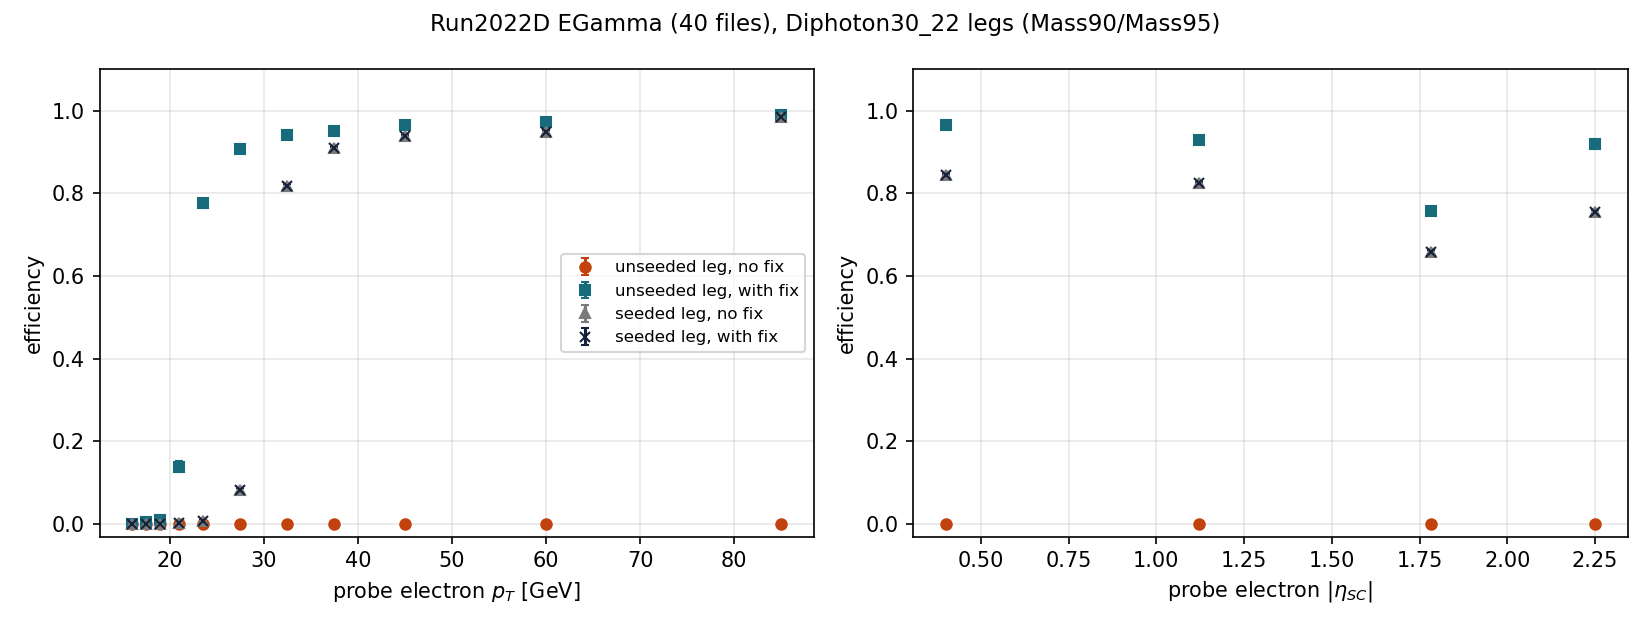
\includegraphics[width=0.98\linewidth,height=0.43\textheight,keepaspectratio]{tnp_compare_2022D_40files_30_22.png}\par\vspace{2pt}
  {\scriptsize
  \begin{tabular}{@{}lll@{}}
    \toprule
    & no fix & with fix\\\midrule
    unseeded leg (bit 14 or 15) & 0 / 59863 & 55133 / 59863 = 0.921 (0.920--0.922)\\
    seeded leg (bit 12 or 13) & 48108 / 59863 = 0.804 & 48108 / 59863 = 0.804, identical in every bin\\\bottomrule
  \end{tabular}}\par\vspace{3pt}
  \whitecap{Z$\to$ee tag-and-probe on NANO re-made in CMSSW\_13\_3\_1\_patch1 from the 40 2022D EGamma 22Sep2023 MINIAOD parents of one central 16Dec2023 NANO file (3125939 events, HTCondor); without the fix the re-made TrigObj equals the central file in 19539 / 19539 shared events.
  Tag: tight e, \pT$>$35, $|\eta_{SC}|<$2.1, HLT\_Ele32\_WPTight\_Gsf object and a seeded-leg photon object. Probe: loose e,
  \pT$>$15, opposite charge, 70$<m_{ee}<$110\,GeV (596 same-sign pairs). 68\% Clopper-Pearson. 2026C data (16\_0\_4\_patch2,
  20000 events): 42 pairs, unseeded leg 0 / 42 without and 39 / 42 with the fix. scripts/tnp\_unseeded.py, scripts/condor/.}
\end{whiteframe}

\begin{whiteframe}{Trigger efficiency with the fix, Diphoton30\_18 (low mass): unseeded leg 0 $\to$ 0.91}
  \centering
  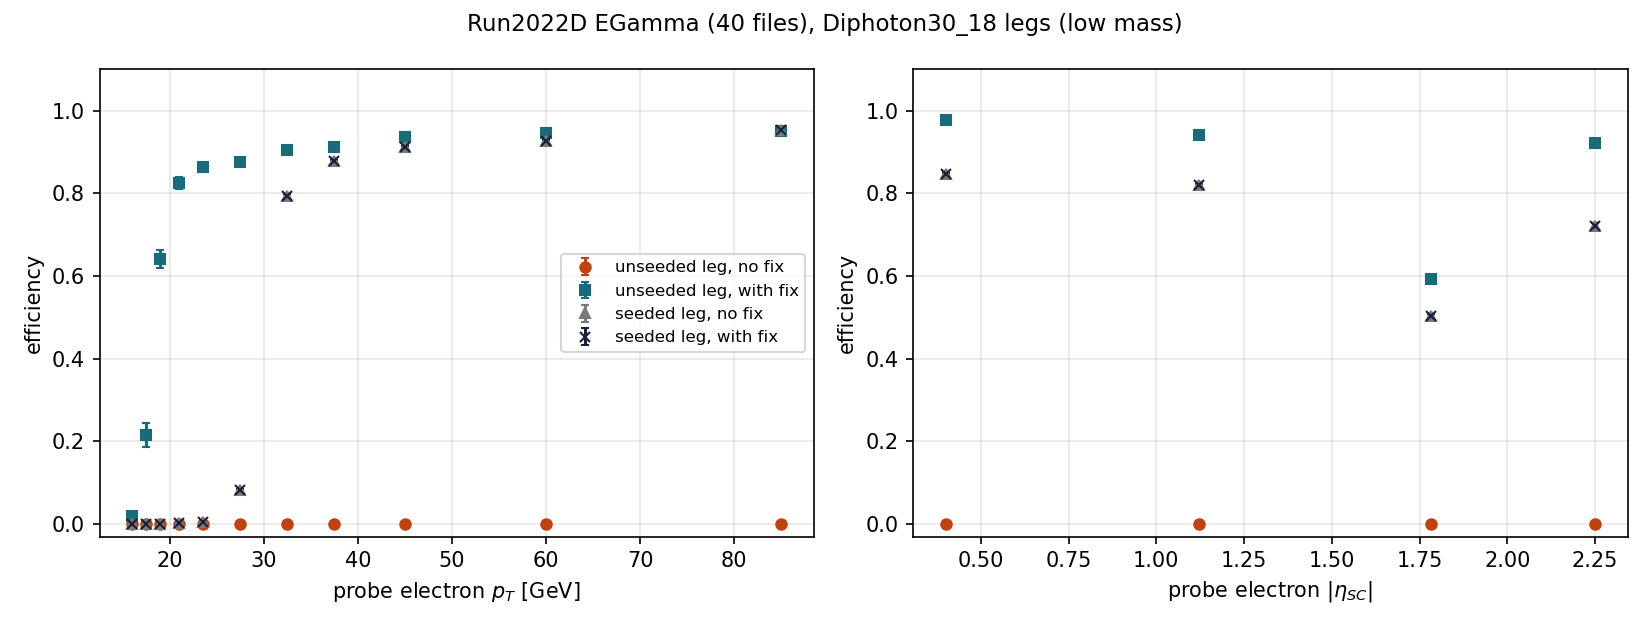
\includegraphics[width=0.98\linewidth,height=0.43\textheight,keepaspectratio]{tnp_compare_2022D_40files_30_18.png}\par\vspace{2pt}
  {\scriptsize
  \begin{tabular}{@{}lll@{}}
    \toprule
    & no fix & with fix\\\midrule
    unseeded leg (EG18 TrackIso, bit 17) & 0 / 57727 & 52460 / 57727 = 0.909 (0.908--0.910)\\
    seeded leg (EG30 EcalIso, bit 16) & 44989 / 57727 = 0.779 & 44989 / 57727 = 0.779, identical in every bin\\\bottomrule
  \end{tabular}}\par\vspace{3pt}
  \whitecap{Same 40 files, tag-and-probe and probe selection as the 30\_22 slide; the tag matches the 30\_18 seeded-leg bit instead
  (537 same-sign pairs). The unseeded-leg turn-on is at 18--20\,GeV here and at 22--25\,GeV for 30\_22. The 1.566--2.0 $|\eta_{SC}|$
  bin is lower for both legs; not investigated. NOTES.md 21; results/tnp\_2022D\_v13\_40files/.}
\end{whiteframe}

\begin{frame}{Relval in CMSSW\_16\_1\_3: the fix builds and runs; these workflows have no TrigObj}
  \vspace{0pt}\par
  {\scriptsize Clean CMSSW\_16\_1\_3 versus the same release with commit 828ed8b2a cherry-picked (one changed line).
  Steps 1--2 ran once; steps 3--4 ran in both areas on the same \code{step2.root}.}
  \par\vspace{6pt}
  {\scriptsize
  \begin{tabularx}{\linewidth}{@{}lYp{1.3cm}p{1.7cm}p{3.3cm}l@{}}
    \toprule
    \thead{workflow} & \thead{content} & \thead{TrigObj in NANO} & \thead{NANO fix vs clean} & \thead{DQM fix vs clean} & \thead{step 3 log}\\\midrule
    12452.0 & H125GGgluonfusion 2023, upgrade matrix, 10 generated events & 0 in both & identical, 10/10 & 116785 histograms; 25 differ, all TimerService & clean\\
    141.046 & EGamma Run2023D run 369978, 100 events, 10 fire Mass90 & 0 in both & identical, 100/100 & 53846 histograms; 25 differ, all TimerService & clean\\\bottomrule
  \end{tabularx}}
  \par\vspace{6pt}
  \begin{itemize}\scriptsize
    \item No \code{Exception} and no \code{triggerObjectTable} line in any step-3 log; outputs identical apart from
          timing histograms.
    \item \gold{The photon selection is not exercised}: the relval HLT summary is nearly empty. In 141.046 the reHLT
          summary is 1428 bytes per event against 34559 for the original 2023 HLT summary of the same file;
          \code{slimmedPatTrigger} is 372 bytes per event. Why was not investigated.
    \item The effect of the fix is therefore shown by the fix test on real MiniAOD input (previous frame).
  \end{itemize}
  \src{results/REPORT.md "Relval in CMSSW\_16\_1\_3"; scripts/relval\_fix\_check.sh and compare\_dqm.py.
  141.046 RAW is on tape only in DAS; one file was read from the IB EOS cache.}
\end{frame}

\begin{frame}{What analyses see, and what HiggsDNA does with the photon bits}
  \begin{itemize}\small
    \item \gold{Datasets}: every Run 3 NanoAOD from v12 on --- 2022 to 2025 data (22Sep2023, 16Dec2023, prompt,
          v15 re-NANO) and the Summer22, 22EE, 23, 23BPix, 24 MC --- plus any Run 2 input re-processed with v12 or later.
    \item \gold{Frameworks}: NanoAOD-based photon matching finds no object for the sub-leading leg. MiniAOD-based
          flashgg reads the PAT objects directly and is unaffected.
    \item \hl{HiggsDNA} (GitLab master d179305; same in ZhenyuDongLL/HiggsDNA-bbggrun3):
      \begin{itemize}\scriptsize
        \item \code{trigger_match} (\code{higgs_dna/utils/misc_utils.py:306}) is called only in
              \code{workflows/dystudies.py:256}, for electrons (pdgid 11, bit 1 or 12).
        \item No workflow tests a photon filter bit or a diphoton filter bit; \code{workflows/lowmass.py:641--642}
              only counts id-11 and id-22 objects.
        \item The low-mass unseeded-leg efficiency comes from a precomputed
              \code{Lowmass_unseeded_leg_efficinecy.json}, whose derivation is not in the repository.
      \end{itemize}
    \item \hl{Elsewhere}: the unseeded filter names appear in 16 files outside cms-sw (analysis legends listing bits
          16 and 17 as the legs, FLAF configurations, custom NanoAOD producers, a flashgg MiniAOD script).
    \item Existing files cannot be repaired: the unseeded objects were never written.
  \end{itemize}
  \src{NOTES.md sections 9 and 13.5 (GitHub code search, default branches only).}
\end{frame}

\begin{frame}{Pull request status and the follow-ups kept out of the one-line fix}
  \begin{columns}[T]
    \begin{column}{0.47\linewidth}
      \hl{Pull request} (prepared, not opened)
      \begin{itemize}\scriptsize
        \item Title: \emph{NanoAOD: accept unseeded e/gamma trigger objects in the Photon TrigObj selection}.
        \item From santanumahata:nano-photon-trigobj-unseeded (828ed8b2a on master ed35654b1) to cms-sw:master;
              xpog signature.
        \item Cites PR 40711 (bits added) and PR 41827 (electrons fixed).
        \item Backport to CMSSW\_15\_0\_X if another production from that branch is planned.
        \item Both branches are on the fork; nothing pushed to cms-sw/cmssw; no pull request exists.
        \item Text: pr/PR\_body.md of the notes branch.
      \end{itemize}
    \end{column}
    \begin{column}{0.51\linewidth}
      \gold{Follow-ups, each a separate pull request}
      \begin{itemize}\scriptsize
        \item 2023 names of the Diphoton30\_18 filters as OR alternatives inside bits 18 and 19.
        \item Move bit 8 (hltHtEcal800) out of the Photon list, or drop it: its objects are HT objects.
        \item Say in the documentation which menus each bit covers; review the stale bits per year.
        \item Photon bits for the low-mass eta1p5, DiphotonMVA14p25, Diphoton15\_1x EBEB and DoublePhoton paths,
              with the EGM POG and the Higgs PAG.
        \item Tell XPOG that MET trigger objects are never written and that the BoostedTau table was empty in v12--v14.
      \end{itemize}
    \end{column}
  \end{columns}
  \src{NOTES.md sections 8.2 and 13.6.}
\end{frame}

\begin{frame}{Summary}
  \begin{itemize}
    \item The Photon trigger-object selection accepts only \code{hltEgammaCandidates}; the sub-leading leg of the
          Diphoton30\_22 Mass90/Mass95 paths lives on \code{hltEgammaCandidatesUnseeded}. Its bits are
          \gold{documented but can never be set}.
    \item Affects \gold{NanoAOD v12, v13, v14, v15 and master}; all HLT menus 2018--2026. Measured on thirteen files
          (incl. 2026 data, 16\_0\_X): 0 photon objects with an unseeded bit in 2.0 million events.
    \item \hl{One-line fix}, the Electron construct of PR 41827. On real MiniAOD input it sets the unseeded bits in
          \hl{all 10453} Mass90 events (\pT\ $\geq$ 22.04\,GeV) and changes no other object; in 2026 data (16\_0\_X) in \hl{all 308}.
    \item Relval in 16\_1\_3: builds and runs cleanly, outputs unchanged; those workflows carry no trigger objects.
    \item Next: open the pull request against cms-sw:master; four follow-ups kept separate.
  \end{itemize}
\end{frame}

% =============================================================
\partdivider{}{Backup}
% =============================================================

\begin{frame}[fragile]{Backup: the path and its sequence in the NanoAOD v13 release menu}
\begin{lstlisting}
# CMSSW_13_3_1_patch1, HLTrigger/Configuration/python/HLT_FULL_cff.py, line 119468 (path) and 118801 (sequence)
fragment.HLT_Diphoton30_22_R9Id_OR_IsoCaloId_AND_HE_R9Id_Mass90_v19 = cms.Path(
    fragment.HLTBeginSequence + fragment.hltL1sSingleAndDoubleEGor
  + fragment.hltPreDiphoton3022R9IdORIsoCaloIdANDHER9IdMass90
  + fragment.HLTDiphoton30L22R9Id85b90eORIso60CaloId15b35eANDHE12R9Id50b80eSequence
  + fragment.hltDiEG22R9Id85b90eORIso60CaloId15b35eANDHE12R9Id50b80eMass90CombMassLastFilter
  + fragment.HLTEndSequence )
# the sequence, e/gamma modules only; cms.ignore(f) = f is run and saves its objects but cannot stop the path
hltEgammaCandidates > hltEGL1SingleAndDoubleEGOrFilter > hltEG30L1SingleAndDoubleEGOrEtFilter
  > hltEG30LR9Id50b80eR9IdFilter > hltEG30LHE12R9Id50b80eHEFilter
  > ignore(hltEG30LR9Id85b90eHE12R9Id50b80eR9IdLastFilter)                     # bit 14
  > ignore(hltEG30LCaloId15b35eHE12R9Id50b80eClusterShapeFilter)
  > ignore(hltEG30LIso60CaloId15b35eHE12R9Id50b80eEcalIsoLastFilter)           # bit 15
  > hltEG30LRId85ORIso60CaloId15b35eANDHE12R9Id50b80eLegCombLastFilter
hltEgammaCandidatesUnseeded > hltDiEG22EtEta2p55UnseededFilter
  > hltDiEG22R9Id50b80eR9IdUnseededFilter > hltDiEG22HE12R9Id50b80eHEUnseededFilter
  > ignore(hltEG22R9Id85b90eHE12R9Id50b80eR9UnseededLastFilter)                # bit 17
  > ignore(hltEG22CaloId15b35eHE12R9Id50b80eClusterShapeUnseededFilter)
  > ignore(hltEG22Iso60CaloId15b35eHE12R9Id50b80eEcalIsoUnseededFilter)
  > ignore(hltEG22Iso60CaloId15b35eHE12R9Id50b80eTrackIsoUnseededLastFilter)   # bit 16
\end{lstlisting}
  \src{Variable producers between the filters are omitted. The path version changes from menu to menu (v13 in 2018,
  v29 in the frozen 2026 menu); the e/gamma filter chain does not (same MD5 in all nineteen menu files).}
\end{frame}

\begin{frame}[fragile]{Backup: the two unseeded last filters, collection explicit in \texttt{l1EGCand}}
  \begin{columns}[T]
    \begin{column}{0.49\linewidth}
\begin{lstlisting}
# bit 17 (v12 to v14: bit 15), trimmed
fragment.hltEG22R9Id85b90eHE12R9Id50b80e
  R9UnseededLastFilter = cms.EDFilter(
  "HLTEgammaGenericFilter",
  saveTags = cms.bool( True ),
  candTag = cms.InputTag(
    "hltDiEG22HE12R9Id50b80eHEUnseededFilter" ),
  varTag = cms.InputTag( 'hltEgammaR9IDUnseeded', 'r95x5' ),
  lessThan = cms.bool( False ),
  useEt = cms.bool( False ),
  thrRegularEB = cms.vdouble( 0.85 ),
  thrRegularEE = cms.vdouble( 0.9 ),
  ncandcut = cms.int32( 1 ),
  l1EGCand = cms.InputTag(
    "hltEgammaCandidatesUnseeded" ) )
\end{lstlisting}
    \end{column}
    \begin{column}{0.49\linewidth}
\begin{lstlisting}
# bit 16 (v12 to v14: bit 14), trimmed
fragment.hltEG22Iso60CaloId15b35eHE12R9Id50b80e
  TrackIsoUnseededLastFilter = cms.EDFilter(
  "HLTEgammaGenericQuadraticFilter",
  saveTags = cms.bool( True ),
  candTag = cms.InputTag( "hltEG22Iso60CaloId15b35e
    HE12R9Id50b80eEcalIsoUnseededFilter" ),
  varTag = cms.InputTag( "hltEgammaHollowTrackIsoUnseeded" ),
  lessThan = cms.bool( True ),
  useEt = cms.bool( True ),
  thrRegularEB = cms.vdouble( 6.0 ),
  thrRegularEE = cms.vdouble( 6.0 ),
  thrOverEEB = cms.vdouble( 0.002 ),
  thrOverEEE = cms.vdouble( 0.002 ),
  ncandcut = cms.int32( 1 ),
  l1EGCand = cms.InputTag(
    "hltEgammaCandidatesUnseeded" ) )
\end{lstlisting}
    \end{column}
  \end{columns}
  \par\vspace{4pt}
  {\scriptsize \code{candTag}: previous filter of the chain; \code{varTag}: variable producer; \code{l1EGCand}: the
  collection the filter tags its saved objects with. The seeded last filters are identical in structure with
  \code{l1EGCand = hltEgammaCandidates}.}
\end{frame}

\begin{frame}[fragile]{Backup: why the unseeded objects carry type 92 (first filter of the leg)}
  \begin{columns}[T]
    \begin{column}{0.46\linewidth}
\begin{lstlisting}
# menu: the first unseeded filter
fragment.hltDiEG22EtEta2p55UnseededFilter =
  cms.EDFilter( "HLT1Photon",
  saveTags = cms.bool( True ),
  inputTag = cms.InputTag( "hltEgammaCandidatesUnseeded" ),
  triggerType = cms.int32( 92 ),
  MinPt = cms.double( 22.0 ),
  MaxEta = cms.double( 2.55 ),
  MinN = cms.int32( 2 ) )
\end{lstlisting}
    \end{column}
    \begin{column}{0.52\linewidth}
\begin{lstlisting}[language=C++]
// HLTrigger/HLTfilters/plugins/HLTSinglet.cc
template <typename T>
int getObjectType(const T&) { return 0; }
// no specialisation for RecoEcalCandidate
if (saveTags())
  filterproduct.addCollectionTag(inputTag_);
...
int tid = getObjectType<T>(*i);
if (tid == 0)
  tid = triggerType_;  // 92, TriggerCluster
filterproduct.addObject(tid, ref);
\end{lstlisting}
    \end{column}
  \end{columns}
  \par\vspace{4pt}
  \begin{itemize}\scriptsize
    \item Every candidate of \code{hltEgammaCandidatesUnseeded} with $E_\mathrm{T}>22$\,GeV is saved with type 92 and
          that collection tag. On the seeded leg the L1-match and $E_\mathrm{T}$ filters save TriggerCluster as well.
    \item \code{type(92)} in NanoAOD is satisfied on both legs: the type is not what rejects the unseeded objects.
  \end{itemize}
  \src{TriggerTypeDefs.h: TriggerPhoton = 81, TriggerCluster = 92, TriggerL1EG = $-98$.}
\end{frame}

\begin{frame}[fragile]{Backup: what the later filters save (\texttt{HLTGenericFilter})}
\begin{lstlisting}[language=C++]
// HLTrigger/Egamma/plugins/HLTGenericFilter.cc (master lines 28 to 32 and 139 to 159; same logic from 10_6_X on)
l1EGTag_ = iConfig.template getParameter<edm::InputTag>("l1EGCand");
...
if (saveTags()) {
  filterproduct.addCollectionTag(l1EGTag_);  // hltEgammaCandidatesUnseeded for the unseeded leg
}
// Set output format
int trigger_type = trigger::TriggerCluster;
if (saveTags())
  trigger_type = trigger::TriggerPhoton;          // 81 for every saved object
...
PrevFilterOutput->getObjects(TriggerCluster, recoCands);
if (recoCands.empty())
  PrevFilterOutput->getObjects(TriggerPhoton, recoCands);  // accepts either type from the previous filter
\end{lstlisting}
  \begin{itemize}\scriptsize
    \item \hl{Collection}: the saved reference points into the \code{l1EGCand} collection; PAT turns it into the label
          \code{hltEgammaCandidatesUnseeded::HLT}.
    \item \hl{Type}: these filters save 81; the object keeps the 92 of the first filter, because PAT attaches the
          type of every filter that accepted it.
    \item Same three statements in 10\_6\_X, 12\_4\_X, 12\_6\_X, 13\_0\_X, 13\_3\_X, 14\_0\_X, 15\_0\_X and master;
          HLTEgammaGenericQuadraticFilter.cc has the identical block (lines 118 to 135).
  \end{itemize}
\end{frame}

\begin{frame}[fragile]{Backup: trigger summary and PAT keep collection label, all types, all filter labels}
  \begin{columns}[T]
    \begin{column}{0.40\linewidth}
\begin{lstlisting}
# menu: the summary producer
fragment.hltTriggerSummaryAOD = cms.EDProducer(
  "TriggerSummaryProducerAOD",
  throw = cms.bool( False ),
  processName = cms.string( "@" ),
  moduleLabelPatternsToMatch = cms.vstring( 'hlt*' ),
  moduleLabelPatternsToSkip = cms.vstring( ) )
\end{lstlisting}
      {\scriptsize Every filter with saveTags contributes; objects are stored once per collection tag, each filter
      records the keys of its objects and the type it saved them with.}
    \end{column}
    \begin{column}{0.58\linewidth}
\begin{lstlisting}[language=C++]
// PhysicsTools/PatAlgos/plugins/PATTriggerProducer.cc (master 680 to 731)
for (size_t iK = 0; iK < keys.size(); ++iK) {
  filterLabels.insert({keys[iK], nameFilter});
  objectTypes.insert({keys[iK], types[iK]});  // per filter
}
...
triggerObject.setCollection(
    handleTriggerEvent->collectionTagEncoded(iC));
for (auto t = objectTypes.equal_range(iO); ...)
  triggerObject.addTriggerObjectType(t.first->second);
...
triggerObjectStandAlone.addFilterLabel(frange.first->second);
triggerObjectStandAlone.addPathName(iP->pathName, ...);
\end{lstlisting}
    \end{column}
  \end{columns}
  \par\vspace{4pt}
  {\scriptsize \code{setCollection} stores \code{hltEgammaCandidatesUnseeded::HLT} for the sub-leading leg; the object
  carries 92 and 81 and every filter label. patTrigger has \code{onlyStandAlone = False} and no excluded collections:
  nothing from the unseeded collection is lost here.}
\end{frame}

\begin{frame}[fragile]{Backup: MiniAOD slims the objects but keeps the collection name}
  \begin{columns}[T]
    \begin{column}{0.32\linewidth}
\begin{lstlisting}[basicstyle=\ttfamily\fontsize{5.3}{6.3}\selectfont\color{offwhite}]
# selectedPatTrigger_cfi.py
selectedPatTrigger = cms.EDFilter(
  "PATTriggerObjectStandAloneSelector",
  src = cms.InputTag("patTrigger"),
  cut = cms.string("!filterLabels.empty()")
)
\end{lstlisting}
      {\scriptsize Keeps every object accepted by at least one saveTags filter.}
    \end{column}
    \begin{column}{0.32\linewidth}
\begin{lstlisting}[basicstyle=\ttfamily\fontsize{5.3}{6.3}\selectfont\color{offwhite}]
# slimmedPatTrigger_cfi.py
slimmedPatTrigger = cms.EDProducer(
  "PATTriggerObjectStandAloneSlimmer",
  src = cms.InputTag("selectedPatTrigger"),
  triggerResults =
    cms.InputTag( 'TriggerResults::HLT' ),
  packFilterLabels = cms.bool(True),
  packP4 = cms.bool(True),
)
\end{lstlisting}
      {\scriptsize Packs four-vector and filter labels; collection string and types stored as they are.}
    \end{column}
    \begin{column}{0.32\linewidth}
\begin{lstlisting}[basicstyle=\ttfamily\fontsize{5.3}{6.3}\selectfont\color{offwhite}]
# NanoAOD triggerObjects_cff.py, 8 to 12
unpackedPatTrigger = cms.EDProducer(
  "PATTriggerObjectStandAloneUnpacker",
  patTriggerObjectsStandAlone =
    cms.InputTag('slimmedPatTrigger'),
  triggerResults =
    cms.InputTag('TriggerResults::HLT'),
  unpackFilterLabels = cms.bool(True)
)
\end{lstlisting}
      {\scriptsize Restores the labels so that \code{filter('...')} can be evaluated.}
    \end{column}
  \end{columns}
  \src{From MiniAOD on the object is a pat::TriggerObjectStandAlone: packed four-vector, collection string, type
  list, packed filter labels, path names.}
\end{frame}

\begin{frame}[fragile]{Backup: the NanoAOD Photon selection --- one collection in \texttt{sel}, three unseeded filters in the bit list}
\begin{lstlisting}
# PhysicsTools/NanoAOD/python/triggerObjects_cff.py, master lines 88 to 116 (v13: 81 to 108), abbreviated
Photon = cms.PSet(
  id = cms.int32(22),
  sel = cms.string("type(92) && pt > 15 && coll('hltEgammaCandidates')"),
  l1seed = cms.string("type(-98)"),  l1deltaR = cms.double(0.3),
  skipObjectsNotPassingQualityBits = cms.bool(True),
  qualityBits = cms.VPSet(
    mksel("filter('hltEG33L1EG26HEFilter')","hltEG33L1EG26HEFilter"),                         # bit 0
    ...  # bits 1 to 13: HE filters, hltHtEcal800, EB tight-ID filters, Mu17_Photon30 photon leg
    mksel("filter('hltEG30LR9Id85b90eHE12R9Id50b80eR9IdLastFilter')", ...),                     # 14
    mksel("filter('hltEG30LIso60CaloId15b35eHE12R9Id50b80eEcalIsoLastFilter')", ...),           # 15
    mksel("filter('hltEG22Iso60CaloId15b35eHE12R9Id50b80eTrackIsoUnseededLastFilter')", ...),   # 16
    mksel("filter('hltEG22R9Id85b90eHE12R9Id50b80eR9UnseededLastFilter')", ...),                # 17
    mksel("filter('hltEG30Iso60CaloId15b35eR9Id50b90eHE12b10eR9Id50b80eEcalIsoFilter')", ...),  # 18
    mksel("filter('hltEG18TrackIso60Iso60CaloId15b35eR9Id50b90eHE12b10eR9Id50b80eTrackIsoUnseededFilter')", ...),  # 19
    mksel("filter('hltEG*L1VBFLooseIsoEGHEFilter')", "hltEG*L1VBFLooseIsoEGHEFilter"),          # 20
  )
),
\end{lstlisting}
  \begin{itemize}\scriptsize
    \item \code{mksel} turns a filter name into \code{filter('name')}, a list into an OR, a tuple into an AND; bit $i$
          is the position in the VPSet.
    \item The contradiction is inside this one PSet: \code{sel} admits only \code{hltEgammaCandidates}, while bits 16,
          17, 19 name filters that run only on \code{hltEgammaCandidatesUnseeded}. No era modifier touches this block.
    \item In v12 to v14 the list has 18 entries (diphoton filters at 12--17); the 21-entry list and 64-bit
          filterBits arrived in CMSSW\_15\_0\_2 (PR 47601, backport of PR 47594).
  \end{itemize}
\end{frame}

\begin{frame}[fragile]{Backup: the table producer --- selection first, bits second, duplicates merged last}
  \begin{columns}[T]
    \begin{column}{0.49\linewidth}
\begin{lstlisting}[language=C++]
// TriggerObjectTableProducer.cc, constructor, lines 105 to 118
for (size_t i = 0; i != cfg.size(); ++i) {
  unsigned int bit = i;
  if (cfg[i].existsAs<unsigned int>("bit"))
    bit = cfg[i].getParameter<unsigned int>("bit");
  assert(!bits[bit] && "...inserted twice");
  assert(bit < 64 && "...on 64 bits");
  func << std::to_string(1UL << bit) << "*("
       << cfg[i].getParameter<std::string>("selection") << ")";
}
qualityBits = StringObjectFunction<...>(func.str());
\end{lstlisting}
    \end{column}
    \begin{column}{0.49\linewidth}
\begin{lstlisting}[language=C++]
// produce(), master lines 151 to 176 (abridged)
for (const auto &obj : trigObjs) {
  for (const auto &sel : sels_) {
    if (sel.match(obj)) {          // fails here
      bits = sel.qualityBits(obj);
      if (skip ? (bits != 0) : true)
        selected.emplace_back(&obj, &sel);
    }
  }
}
// Self-cleaning
for (i ...) for (j < i ...)
  if (sel.id == sel2.id && deltaR2(obj, obj2) < 1e-6) {
    bits_of(obj2) |= bits_of(obj);
    selected.erase(selected.begin() + i); i--;
  }
\end{lstlisting}
    \end{column}
  \end{columns}
  \par\vspace{4pt}
  \begin{itemize}\scriptsize
    \item \gold{Order of evaluation is the whole story}: an object that fails \code{sel} never reaches the bits, never
          enters \code{selected}, and is never seen by the merging loop.
    \item Since 13\_0\_X an object is tested against every selection (it can be both id 11 and id 22); 12\_4\_X had a
          \code{break} after the first match.
  \end{itemize}
\end{frame}

\begin{frame}{Backup: the producer changed three times since 2022; selection-before-bits never did}
  \vspace{0pt}\par
  {\scriptsize
  \begin{tabularx}{\linewidth}{@{}Yllp{4.0cm}l@{}}
    \toprule
    \thead{releases (NanoAOD)} & \thead{filterBits} & \thead{bit limit} & \thead{duplicate merging} & \thead{selections per object}\\\midrule
    12\_4\_X, 12\_6\_X (v10, v11) & Int\_t & bit $<$ 31 & same id, same \pT, same direction & first match only (break)\\
    13\_0\_X to 14\_2\_X, 15\_0\_0, 15\_0\_1 (v12--v14) & Int\_t & bit $<$ 31 & same id, $|\Delta\pT|<10^{-6}$, $\Delta R^2<10^{-6}$ (\pT\ test dropped in 15\_0\_0) & every matching selection\\
    15\_0\_2 onward, master (v15, next) & uint64 & bit $<$ 64 & same id, $\Delta R^2<10^{-6}$ & every matching selection\\\bottomrule
  \end{tabularx}}
  \par\vspace{8pt}
  \begin{itemize}\small
    \item In every version \code{sel.match(obj)} is tested first; only a passing object gets its bits.
    \item The merging rule only matters after the fix: a seeded and an unseeded object describing the same photon
          merge on direction alone with the master rule.
  \end{itemize}
  \src{Checked at the tags 14\_1\_0, 14\_2\_0, 15\_0\_0, 15\_0\_1, 15\_0\_2, 15\_0\_5, 15\_0\_10, 15\_0\_13, 15\_0\_15,
  15\_0\_15\_patch4, 15\_1\_0, 16\_0\_0 and the tips of 12\_4\_X, 13\_0\_X, 14\_0\_X, 15\_0\_X. The 64-bit change matches
  PR 47594 / 47601, merged 18 March 2025.}
\end{frame}

\begin{frame}[fragile]{Backup: how \texttt{coll('hltEgammaCandidates')} is evaluated --- no star, exact label comparison}
  \begin{columns}[T]
    \begin{column}{0.49\linewidth}
\begin{lstlisting}[language=C++]
// DataFormats/PatCandidates/src/TriggerObjectStandAlone.cc
bool TriggerObjectStandAlone::hasCollection(
    const std::string &collName) const {
  // Move to wild-card parser, if needed only
  if (collName.find(wildcard_) != std::string::npos) {
    if (hasAnyName(collName, {collection()}))
      return true;
    ...  // label / instance / process with wildcards
    return false;
  }
  // Use parent class's method otherwise
  return TriggerObject::hasCollection(collName);
}
\end{lstlisting}
    \end{column}
    \begin{column}{0.49\linewidth}
\begin{lstlisting}[language=C++]
// DataFormats/PatCandidates/src/TriggerObject.cc, 54 to 71
bool TriggerObject::hasCollection(
    const std::string& collName) const {
  if (collName == collection_) return true;
  const edm::InputTag collectionTag(collection_);
  const edm::InputTag collTag(collName);
  if (collTag.process().empty()) {
    if ((collTag.instance().empty()
        && collectionTag.instance().empty())
        || collTag.instance() == collectionTag.instance()) {
      return (collTag.label() == collectionTag.label());
    }
  }
  return false;
}
\end{lstlisting}
    \end{column}
  \end{columns}
  \par\vspace{4pt}
  {\scriptsize For the unseeded object: \code{collName = hltEgammaCandidates},
  \code{collection_ = hltEgammaCandidatesUnseeded::HLT}. No star, so the base method runs; the labels differ; the result
  is false. \code{filter('...')} behaves the same way through \code{hasFilterOrCondition}.}
\end{frame}

\begin{frame}{Backup: six other explanations, and the evidence that rules each one out}
  \vspace{0pt}\par
  {\scriptsize
  \begin{tabularx}{\linewidth}{@{}p{3.6cm}Yl@{}}
    \toprule
    \thead{hypothesis} & \thead{what the code and the menus show} & \thead{verdict}\\\midrule
    Filter names misspelt or outdated & All four Diphoton30\_22 names defined with saveTags = True in the 2018, 2022 v1.2/v1.4/v1.5, 2023, 2024, 2025, 2026 menus and every development menu checked (19 files); chain identical & ruled out\\
    Unseeded objects never reach MiniAOD & patTrigger excludes no collection; selectedPatTrigger keeps objects with any filter label; the Electron selection consumes the unseeded collection in production since June 2023 & ruled out\\
    Wrong type for \code{type(92)} & HLT1Photon saves them with triggerType 92; the later filters add 81; PAT keeps both & ruled out\\
    The \pT\ threshold removes them & sel requires pt $>$ 15; the leg requires 22\,GeV (18\,GeV for Diphoton30\_18) & ruled out\\
    An era modifier changes the Photon block & Modifiers act on Muon, Tau, Jet (Run 2 eras) and the prefiring producer; none on Photon & ruled out\\
    Specific to the v13 release & 13\_3\_1\_patch1 and the 13\_3\_X tip are byte-identical; 13\_0\_X to master carry the same selection & ruled out\\
    \rowdead The Photon selection rejects the collection & \code{coll('hltEgammaCandidates')}, exact comparison, before the bits & \dead{the cause}\\\bottomrule
  \end{tabularx}}
  \src{NOTES.md section 7.1.}
\end{frame}

\begin{frame}[fragile]{Backup: why not a wildcard, and exactly which objects the fix lets through}
  \begin{columns}[T]
    \begin{column}{0.47\linewidth}
\begin{lstlisting}[language=C++]
// TriggerObjectStandAlone::hasAnyName, lines 80 to 119 (abridged)
boost::split(parts, name, is_any_of("*"), token_compress_on);
for (name in nameVec) {
  index = 0;
  for (part in parts) {
    if (part.empty()) continue;
    index = name.find(part, index);
    if (index == npos ||
        (part is first && index > 0)) { failed; break; }
    index += part.length();
  }
  // Failed, if end of name not reached
  if (index < name.length() && !parts.back().empty())
    failed = true;
}
\end{lstlisting}
    \end{column}
    \begin{column}{0.51\linewidth}
      {\tiny
      \begin{tabularx}{\linewidth}{@{}Yll@{}}
        \toprule
        \thead{unseeded filter that is a photon bit} & \thead{bit} & \thead{menus}\\\midrule
        \fname{hltEG22Iso60CaloId15b35eHE12R9Id50b80eTrackIsoUnseededLastFilter} & 16 & 2018--2026\\
        \fname{hltEG22R9Id85b90eHE12R9Id50b80eR9UnseededLastFilter} & 17 & 2018--2026\\
        \fname{hltEG18TrackIso60Iso60CaloId15b35eR9Id50b90eHE12b10eR9Id50b80eTrackIsoUnseededFilter} & 19 & 2018, 2022\\\bottomrule
      \end{tabularx}}
      \par\vspace{4pt}
      {\scriptsize The only photon-list entries whose filters run on the unseeded collection (nine menus checked;
      the wildcard bit 20 matches only the seeded \code{hltEG22L1VBFLooseIsoEGHEFilter}). Other unseeded e/gamma
      objects set no photon bit and are dropped by the skip flag.}
    \end{column}
  \end{columns}
  \src{\code{coll('hltEgammaCandidates*')} would match both collections. The anchoring rule is also what kills the
  v12--v14 BoostedTau pattern (no trailing star, name continues).}
\end{frame}

\begin{frame}[fragile]{Backup: the breadth scan --- every filter bit of every object type against each menu}
\begin{lstlisting}[language=Python]
# scripts/deadbits.py (notes repository), the core
def glob_re(pat):  # NanoAOD wildcard semantics
  parts = pat.split("*")
  return re.compile("^" + ".*".join(re.escape(p) for p in parts) + "$")
def collections_of(mods, name):
  # EDProducer labels a filter saves its objects from
  typ, body = mods[name]
  for p in ("l1EGCand", "inputTag", "CandTag", "inputCandCollection", "originTag1", ...):
    for lab in tag_labels(body, p):
      if mods[lab][0] == "EDProducer": direct.add(lab)
      elif mods[lab][0] == "EDFilter": follow.append(lab)
  return direct or union(collections_of(mods, f) for f in follow)
status = OK if any matched filter's collection passes coll()
        else COLL if filters match but none passes
        else STALE if no module matches the pattern
\end{lstlisting}
  \begin{itemize}\scriptsize
    \item \hl{Inputs}: configs master, 15\_0\_X (v15), 13\_3\_1\_patch1 (v13), 13\_0\_13 (v12); frozen menus 2022 v1.2
          and v1.4, 2023 v1.2, 2024 v1.4, 2025 v1.3, 2026 v1.3 and the GRun menus of 13\_0\_X, 14\_0\_X, 15\_0\_X, 16\_1\_X.
    \item \hl{Emulates} mksel, the anchored star matching of hasAnyName, the collection each matched filter saves and the
          \code{coll()} terms. The type test is not emulated; Tau's \code{coll('*Tau*')} is treated as non-restrictive.
  \end{itemize}
\end{frame}

\begin{frame}[fragile]{Backup: three more entries that can never be filled}
  \begin{columns}[T]
    \begin{column}{0.32\linewidth}
      \gold{Photon bit 8: hltHtEcal800}
\begin{lstlisting}
fragment.hltHtEcal800 = cms.EDFilter(
  "HLTHtMhtFilter",
  saveTags = cms.bool( True ),
  htLabels = cms.VInputTag( 'hltHtMhtEcal' ),
  minHt = cms.vdouble( 800.0 ), ... )
// HLTHtMhtFilter.cc, 104 to 105
addObject(trigger::TriggerTHT, htref);
addObject(trigger::TriggerMHT, mhtref);
\end{lstlisting}
      {\tiny HT objects (types 89, 90): never type 92, never an e/gamma collection. Dead since v10.}
    \end{column}
    \begin{column}{0.32\linewidth}
      \gold{MET: no bits, skip flag on}
\begin{lstlisting}
MET = cms.PSet(
  id = cms.int32(2),
  sel = cms.string("type(87) && pt > 30
    && coll('hltPFMETProducer')"),
  skipObjectsNotPassingQualityBits
    = cms.bool(True),
  qualityBits = cms.VPSet()
)
\end{lstlisting}
      {\tiny The bit function is the constant 0, so every MET object is dropped: TrigObj has never contained MET,
      although the documentation lists id 2.}
    \end{column}
    \begin{column}{0.32\linewidth}
      \gold{BoostedTau in v12 to v14}
\begin{lstlisting}
# 13_0_X to 15_0_1
sel = "type(85) && pt > 120
  && coll('hltAK8PFJetsCorrected')
  && filter('hltAK8SinglePFJets*
     SoftDropMass40*ParticleNetTauTau')"
# menus: 2022 ...ParticleNetTauTau0p30
#        2023+ ...PNetTauTauTag0p03
# 15_0_2: filter('*TauTau*')
\end{lstlisting}
      {\tiny End-anchored pattern, no menu name matches; jets come from hltAK8PFJets230SoftDropMass40. Relaxed in 15\_0\_2.}
    \end{column}
  \end{columns}
  \src{Side findings of the scan, for XPOG; none changes the photon fix. Measured: no id-2 object in any file;
  BoostedTau objects only in the v15 files (22, 430, 254).}
\end{frame}

\begin{frame}{Backup: stale bits by year --- documented filters that no longer exist in that year's menu}
  \vspace{0pt}\par
  {\tiny
  \begin{tabularx}{\linewidth}{@{}llYll@{}}
    \toprule
    \thead{object} & \thead{bit} & \thead{filter pattern (master list)} & \thead{exists in menus} & \thead{empty for data of}\\\midrule
    Electron & 2 & \code{hltEle*WPLoose*TrackIsoFilter} & 2022 & 2023 onward\\
    Electron & 8 & \code{hltEle*Ele*Ele*CaloIdLTrackIdLDphiLeg*Filter} (3e) & 2022 to 2024 & 2025 onward\\
    Photon & 12 & \code{hltEG120EBTightIDTightIsoTrackIsoFilter} & 2018, early 2022 & 2022 v1.4 onward\\
    Photon & 18, 19 & Diphoton30\_18 filters (hltEG30Iso60... and hltEG18TrackIso60...) & 2018, 2022 & 2023 onward (renamed)\\
    Muon & 2, 6 & \code{*OverlapFilterIsoMu*PFTau*} (DeepTau mu-tau overlap) & 2022 to 2024 & 2025 onward\\
    Tau & 3 & \code{*DeepTau*} & 2022 to 2024 & 2025 onward\\
    BoostedTau & 0 & \code{hltAK8SinglePFJets*SoftDropMass*ParticleNetTauTau0p30} & 2022 & 2023 onward\\
    Jet & 0, 1, 6, 22, 27 & pixel-only PFCentralJetTightID (HH to 4b) & 2022, 2023 & 2024 onward\\
    Jet & 8, 9, 11, 24, 25 & 3PFCentralJetTightIDPt40/45, BTagCaloDeepCSVp17Double, BTagPFDeepJet1p5Single/4p5Triple & 2022 to 2023/2024 & 2023, 2024 or 2025 onward\\
    FatJet & 3, 4, 5 & SoftDropMass40BTagParticleNetBB0p35, AK8DoublePFJetSDModMass30/50 & 2022 (2023 for 4, 5) & 2023 or 2024 onward\\
    HT & 0, 1 & Run 2 L1 seed names & Run 2 only & all Run 3\\\bottomrule
  \end{tabularx}}
  \par\vspace{5pt}
  {\scriptsize Bits added for newer filters are empty for earlier years in the same way. This is the price of one bit
  list for five years of menus, not a code defect; the photon bits are the only ones no menu can cure.}
  \src{Read off the scanner output for the master configuration against the 2022 to 2026 frozen and development menus.}
\end{frame}

\begin{frame}{Backup: photon filter bits 0 to 10 (master numbering)}
  \vspace{0pt}\par
  {\scriptsize
  \begin{tabularx}{\linewidth}{@{}llYll@{}}
    \toprule
    \thead{bit v15} & \thead{bit v12--v14} & \thead{filter} & \thead{objects come from} & \thead{filter exists in}\\\midrule
    0--7 & 0--7 & \fname{hltEG33L1EG26HEFilter}, \fname{hltEG50/75/90/120/150/175/200HEFilter} & hltEgammaCandidates & 2018 to 2026\\
    \rowdead 8 & 8 & \code{hltHtEcal800} & \dead{hltHtMhtEcal (HT object): never a photon} & 2018 to 2026\\
    9 & none & \fname{hltEG45EBTightIDTightIsoTrackIsoFilter} & hltEgammaCandidates & 2024 to 2026\\
    10 & none & \fname{hltEG50EBTightIDTightIsoTrackIsoFilter} & hltEgammaCandidates & 2023 to 2026\\\bottomrule
  \end{tabularx}}
  \par\vspace{6pt}
  {\scriptsize Bits 0 to 7: single-photon H/E filters of the HLT\_Photon paths; 9 to 12: barrel tight-ID isolated
  photon filters; 13: photon leg of Mu17\_Photon30. Only bit 8 is misplaced in this half of the list.}
  \src{triggerObjects\_cff.py at master ed35654b1 (21 entries) and CMSSW\_13\_3\_1\_patch1 (18 entries); "objects come
  from" is the l1EGCand (or htLabels) of the module in the menu.}
\end{frame}

\begin{frame}{Backup: photon filter bits 11 to 20, with the three dead unseeded entries}
  \vspace{0pt}\par
  {\tiny
  \begin{tabularx}{\linewidth}{@{}llYp{3.6cm}l@{}}
    \toprule
    \thead{v15} & \thead{v12--v14} & \thead{filter} & \thead{objects come from} & \thead{filter exists in}\\\midrule
    11 & 9 & \fname{hltEG110EBTightIDTightIsoTrackIsoFilter} & hltEgammaCandidates & 2018 to 2026\\
    12 & 10 & \fname{hltEG120EBTightIDTightIsoTrackIsoFilter} & hltEgammaCandidates & 2018, 2022 v1.2 only\\
    13 & 11 & \fname{hltMu17Photon30IsoCaloIdPhotonlegTrackIsoFilter} & hltEgammaCandidates & 2018 to 2026\\
    14 & 12 & \fname{hltEG30LR9Id85b90eHE12R9Id50b80eR9IdLastFilter} & hltEgammaCandidates & 2018 to 2026\\
    15 & 13 & \fname{hltEG30LIso60CaloId15b35eHE12R9Id50b80eEcalIsoLastFilter} & hltEgammaCandidates & 2018 to 2026\\
    \rowdead 16 & 14 & \fname{hltEG22Iso60CaloId15b35eHE12R9Id50b80eTrackIsoUnseededLastFilter} & \dead{hltEgammaCandidatesUnseeded, never set} & 2018 to 2026\\
    \rowdead 17 & 15 & \fname{hltEG22R9Id85b90eHE12R9Id50b80eR9UnseededLastFilter} & \dead{hltEgammaCandidatesUnseeded, never set} & 2018 to 2026\\
    18 & 16 & \fname{hltEG30Iso60CaloId15b35eR9Id50b90eHE12b10eR9Id50b80eEcalIsoFilter} & hltEgammaCandidates & 2018, 2022 (renamed 2023)\\
    \rowdead 19 & 17 & \fname{hltEG18TrackIso60Iso60CaloId15b35eR9Id50b90eHE12b10eR9Id50b80eTrackIsoUnseededFilter} & \dead{hltEgammaCandidatesUnseeded, never set} & 2018, 2022 (renamed 2023)\\
    20 & none & \fname{hltEG*L1VBFLooseIsoEGHEFilter} (only hltEG22L1VBFLooseIsoEGHEFilter) & hltEgammaCandidates & 2023 to 2026\\\bottomrule
  \end{tabularx}}
  \src{From 2023 the Diphoton30\_18 filters are called hltEG30Iso60b40eCaloId11b32eHE10b9eR9Id50b90eEcalIsoFilter and
  hltDiEG18TrackIso60Iso60b40eCaloId11b32eHE10b9eR9Id50b90eTrackIsoUnseededFilter, so bits 18 and 19 match nothing for
  2023 and later data.}
\end{frame}

\begin{frame}{Backup: how the defect was born, survived and was found}
  \begin{itemize}\small
    \item \gold{7--8 Feb 2023}: PR 40711 adds the six diphoton photon bits for the next NanoAOD production. The Photon
          selection is not touched: the three unseeded bits are dead from day one (CMSSW\_13\_0\_0; v12 made with 13\_0\_13).
    \item \gold{31 May -- 8 Jun 2023}: PR 41827 gives the Electron selection the unseeded collection and the CaloIdL\_MW
          unseeded bit. Photons are not revisited. In CMSSW\_13\_3\_0, so v13 has it for electrons only.
    \item \gold{Nov -- Dec 2023}: 13\_3\_X backports for v13 (43292 from 43247, 43286, 43470 and others);
          CMSSW\_13\_3\_1\_patch1 produces v13 for Summer22, 22EE, 23, 23BPix MC and the 16Dec2023 2022 data.
    \item \gold{13--18 Mar 2025}: PR 47594 / 47601 add hltEG45 and hltEG50 EB bits and the VBF wildcard; filterBits
          becomes 64-bit (CMSSW\_15\_0\_2). The unseeded bits move to 16, 17, 19, still dead. v15 inherits them.
    \item \gold{4 Nov 2026}: cause located, confirmed on master and the 16\_x branches, whole-table scan, fix committed,
          ten files measured on lxplus.
    \item \gold{5 Nov 2026}: three more files (one 2026, 16\_0\_X); fix test on real MiniAOD input in 13\_3\_1\_patch1,
          15\_0\_15\_patch4 and 16\_0\_4\_patch2; relval in 16\_1\_3.
  \end{itemize}
  \src{Dates are the creation and merge dates from the GitHub search API. Between CMSSW\_13\_0\_0 and 13\_0\_1 the photon
  pt threshold moved from 20 to 15 GeV; that change did not touch the collection test.}
\end{frame}

\begin{frame}{Backup: NanoAOD versions, releases and the v13 production recipe}
  \begin{columns}[T]
    \begin{column}{0.48\linewidth}
      {\tiny
      \begin{tabularx}{\linewidth}{@{}lY@{}}
        \toprule
        \thead{NanoAOD} & \thead{release (evidence as in NOTES.md 3.1)}\\\midrule
        v9 & CMSSW\_10\_6\_X (era modifier run2\_nanoAOD\_106Xv2)\\
        v10 & CMSSW\_12\_4\_X (run3\_nanoAOD\_124)\\
        v11, v11\_1 & CMSSW\_12\_6\_X (reported)\\
        v12 & CMSSW\_13\_0\_X, production 13\_0\_13 (reported)\\
        v13 & CMSSW\_13\_3\_X, production 13\_3\_1\_patch1\\
        v14 & CMSSW\_14\_0\_X (reported)\\
        v15 & CMSSW\_15\_0\_X: $\geq$15\_0\_2 for 2024; 15\_0\_15\_patch4 for 2022/2023 inputs (run3\_nanoAOD\_pre142X)\\
        (v16) & no dataset named v16 in DAS; 2026 PromptReco is CMSSW\_16\_0\_X (16\_0\_2\_patch1 to 16\_0\_5\_patch1)\\\bottomrule
      \end{tabularx}}
    \end{column}
    \begin{column}{0.50\linewidth}
      {\tiny
      \begin{tabularx}{\linewidth}{@{}Yl@{}}
        \toprule
        \thead{v13 MC campaign: global tag} & \thead{era}\\\midrule
        Run3Summer22: 133X\_mcRun3\_2022\_realistic\_ForNanov13\_v1 & Run3\\
        Run3Summer22EE: 133X\_mcRun3\_2022\_realistic\_postEE\_ForNanov13\_v1 & Run3\\
        Run3Summer23: 133X\_mcRun3\_2023\_realistic\_ForNanov13\_v1 & Run3\_2023\\
        Run3Summer23BPix: 133X\_mcRun3\_2023\_realistic\_postBPix\_ForNanov13\_v2 & Run3\_2023\\\bottomrule
      \end{tabularx}}
      \par\vspace{4pt}
      {\tiny Input: 13\_0\_X MiniAODv4. Data: 2022 re-processed from 22Sep2023 MiniAOD as 16Dec2023 (v13); 2023 data
      stays at v12.}
    \end{column}
  \end{columns}
  \par\vspace{6pt}
  {\scriptsize The version of a NanoAOD file is set by the release it was made in plus the era: there is no
  version-specific switch in the code. The file itself tells: 12 photon bits (v10, v11), 18 (v12 to v14),
  21 with a 64-bit \code{filterBits} (v15).}
  \src{NOTES.md sections 3.1 to 3.4; v13 command shape from public configurations that mirror the McM setup.}
\end{frame}

\begin{frame}{Backup: how the thirteen files were measured}
  \begin{itemize}\small
    \item lxplus, Python with uproot and awkward from LCG\_107, files read through \code{root://cms-xrd-global.cern.ch/};
          one file per dataset, the first \code{dasgoclient} returns; up to 300000 events per file.
    \item Bit numbers \hl{parsed from each file's own} \code{TrigObj_filterBits} documentation, never hard-coded.
    \item Counted per file: photon objects with each seeded and unseeded bit (all events and Mass90-fired events),
          electron objects with the CaloIdL\_MW-unseeded bit, objects per TrigObj id, events with any photon
          carrying an unseeded bit (with run, lumi, event of the first 50).
    \item File layout cross-check: 12 photon bits (v10, v11), 18 (v12 to v14), 21 and \code{>u8} (v15).
    \item Documentation curiosities seen in the files: the v10 file lists 11 photon filters (no Mu17\_Photon30 leg);
          the v11 file names bits 5 and 6 both hltEG150HEFilter; the Winter24 file carries 133X and the 18-bit layout.
    \item Not covered: NanoAOD v14 (14\_0\_X) MC is not in DAS.
  \end{itemize}
  \src{scripts/measure\_trigobj.py; one JSON per file under results/; results/REPORT.md.}
\end{frame}

\begin{frame}[fragile]{Backup: the fix test, exactly as run (scripts/make\_fixed\_nano.sh)}
\begin{lstlisting}[language=bash]
INPUT=root://cms-xrd-global.cern.ch//store/mc/Run3Summer23MiniAODv4/GluGluHto2G_M-125_TuneCP5_13p6TeV_amcatnloFXFX-pythia8/
      MINIAODSIM/130X_mcRun3_2023_realistic_v15_ext1-v4/2820000/74338d47-0b38-4e0b-83a2-ad85c7f4e533.root   # parent of central v13 file
# v13: CMSSW_13_3_1_patch1, era Run3_2023,                        GT 133X_mcRun3_2023_realistic_ForNanov13_v1
# v15: CMSSW_15_0_15_patch4, era Run3_2023,run3_nanoAOD_pre142X,  GT 150X_mcRun3_2023_realistic_v1
# v16: CMSSW_16_0_4_patch2, --data, era Run3_2026, GT 160X_dataRun3_Prompt_frozen260223_v1, -n 20000, input below
#      /store/data/Run2026C/EGamma0/MINIAOD/PromptReco-v1/000/402/536/00000/33c652d5-5e17-456b-9b90-6d8e00734855.root
scram project CMSSW $RELEASE; cd $RELEASE/src; eval $(scramv1 runtime -sh)
git cms-addpkg PhysicsTools/NanoAOD; scram b -j 8
cmsDriver.py nano_nofix --step NANO --mc --scenario pp --nThreads 4 --eventcontent NANOAODSIM --datatier NANOAODSIM \
    --conditions $GT --era $ERA --filein $INPUT --fileout file:nano_nofix.root -n -1
sed -i "s#type(92) && pt > 15 && coll('hltEgammaCandidates')\"#type(92) \&\& pt > 15 \&\& (coll('hltEgammaCandidates') || coll('hltEgammaCandidatesUnseeded'))\"#" \
    PhysicsTools/NanoAOD/python/triggerObjects_cff.py
git diff --numstat          # must be exactly "1 1"
scram b -j 8
cmsDriver.py nano_fix  ... same options ... --fileout file:nano_fix.root
python3 measure_trigobj.py v13_nofix ... nano_nofix.root nano_nofix.json <central v13 file>   # event-by-event comparison
python3 measure_trigobj.py v13_fix   ... nano_fix.root   nano_fix.json   nano_nofix.root
\end{lstlisting}
  \begin{itemize}\scriptsize
    \item The MiniAOD dataset first proposed (\code{...realistic_v14-v2/MINIAODSIM}) has 0 files in DAS; the DAS parent of
          the central v13 file was used instead, so the no-fix output can be compared with the central file event by event.
    \item The v15 global tag is the processing string of \code{Run3Summer23NanoAODv15} in DAS (no GluGluH dataset exists there).
    \item The changed line is 83 in 13\_3\_1\_patch1 and 86 in 15\_0\_15\_patch4. One v13 \code{nano_fix} run was
          terminated externally at 8532 events and rerun with the same configuration.
  \end{itemize}
\end{frame}

\begin{frame}{Backup: the relval check in detail}
  \begin{itemize}\small
    \item \hl{Areas}: \code{clean} = CMSSW\_16\_1\_3; \code{fix} = the same release + \code{git cms-addpkg PhysicsTools/NanoAOD}
          + \code{git cherry-pick 828ed8b2a}; \code{git diff CMSSW_16_1_3 --numstat} = one line. Cherry-pick instead of
          \code{git cms-merge-topic}, because the topic branch sits on master, not on the 16\_1\_X release.
    \item \hl{12452.0}: not in the default matrix of 16\_1\_3 (\code{-w upgrade} needed); its RelVal GEN-SIM input returned
          no file at T2\_CH\_CERN, so step 1 generated the 10 events.
    \item \hl{141.046}: run 369978 RAW is on tape only in DAS (T0\_CH\_CERN\_Tape, T1\_US\_FNAL\_Tape); of 321 files listed,
          one is in the IB EOS cache and was used for step 2 (100 events). Steps 3--4 from \code{runTheMatrix --dryRun}.
    \item Step-3 NANO is EDM (NANOEDMAOD); converted to flat NANO with \code{cmsDriver.py --step NONE} before measuring.
    \item \hl{Per-event sizes} (\code{edmEventSize -v}): 141.046 \code{hltTriggerSummaryAOD__reHLT} 1427.78\,B vs
          \code{hltTriggerSummaryAOD__HLT} 34558.6\,B; \code{slimmedPatTrigger__reRECO} 371.96\,B; 12452.0
          \code{hltTriggerSummaryAOD__HLT} 1313\,B.
  \end{itemize}
  \src{scripts/relval\_fix\_check.sh, scripts/compare\_dqm.py; JSONs in results/relval\_16\_1\_3/.}
\end{frame}

\begin{frame}[fragile]{Backup: counting the new bits on any NanoAOD file}
\begin{lstlisting}[language=Python]
# count photon objects with the unseeded bits, per path
import uproot, awkward as ak, numpy as np
t = uproot.open("nano.root")["Events"]
path = "HLT_Diphoton30_22_R9Id_OR_IsoCaloId_AND_HE_R9Id_Mass90"
a = t.arrays(["TrigObj_id", "TrigObj_filterBits", path])
ph    = a["TrigObj_id"] == 22
bits  = ak.values_astype(a["TrigObj_filterBits"][ph], np.uint64)
fired = a[path]
for bit in (16, 17):   # 14, 15 for NanoAOD v12 to v14
  has = ak.any(((bits >> np.uint64(bit)) & np.uint64(1)) == 1, axis=1)
  print(bit, int(np.sum(has & fired)), "of", int(np.sum(fired)))
\end{lstlisting}
  \begin{itemize}\small
    \item Before the fix both counts are 0 by construction. In the fix test every one of the 10453 Mass90 events has a
          photon with at least one of the two bits.
    \item For v12 to v14 files the loop runs over bits 14 and 15 and \code{filterBits} is 32-bit; the uint64 cast is harmless.
  \end{itemize}
  \src{NOTES.md section 8.1; the full measurement is scripts/measure\_trigobj.py.}
\end{frame}

\begin{frame}[fragile]{Backup: what the trigger-object rows look like, today and with the fix}
\begin{lstlisting}
# schematic TrigObj rows of one diphoton-triggered event (illustration of the structure, not real data)
today (v15):
 id  pt     filterBits        meaning
 22  41.7   0x4000 (bit 14)   leading leg, R9 last
 -- no row for the 26 GeV photon --
with the fix:
 22  41.7   0x4000 (bit 14)   leading leg, R9 last
 22  26.3   0x20000 (bit 17)  unseeded leg, R9 last
\end{lstlisting}
  \begin{itemize}\small
    \item A leading photon that also passes the unseeded leg merges with its unseeded twin (same direction) and carries
          both bits; a sub-leading photon appears as a new row.
    \item The rows are made up to show the structure; \pT\ values and row counts differ event by event. The measured
          effect is in the fix-test table: photon objects 24835 $\to$ 26639 for 17760 events (v13).
  \end{itemize}
\end{frame}

\begin{frame}{Backup: where everything is}
  \begin{itemize}\small
    \item \hl{Notes branch}: \url{https://github.com/santanumahata/cmssw/tree/nanoaod-trigobj-notes}
      \begin{itemize}\scriptsize
        \item \code{NOTES.md}: the knowledge base (sections 0 to 16).
        \item \code{results/}: REPORT.md, one JSON per measured file, \code{fix_test/}, \code{relval_16_1_3/}.
        \item \code{scripts/}: measure\_trigobj.py, make\_fixed\_nano.sh, relval\_fix\_check.sh, compare\_dqm.py,
              deadbits.py and the menu scanners.
        \item \code{scan/}: raw scanner outputs; \code{pr/}: patch and PR text; \code{report/}: issue report (PDF);
              \code{slides/}: the HTML decks and this Beamer deck.
      \end{itemize}
    \item \hl{Fix branch}: \url{https://github.com/santanumahata/cmssw/tree/nano-photon-trigobj-unseeded} (828ed8b2a).
    \item \hl{Open the pull request} (creates nothing by itself):\\
          {\scriptsize\url{https://github.com/cms-sw/cmssw/compare/master...santanumahata:cmssw:nano-photon-trigobj-unseeded}}
  \end{itemize}
\end{frame}

\end{document}
